%%%%%%%%%%%%%%%%%%%%%%%%%%%%%%%%%%%%%%%%%%%%%%%%%%%%%%%%%%
% # Appendix: Acceptability Judgment Task Materials
%%%%%%%%%%%%%%%%%%%%%%%%%%%%%%%%%%%%%%%%%%%%%%%%%%%%%%%%%%

\chapter{Acceptability Judgment Task Materials}\label{app-materials-ajt}

Acceptability judgment tasks (AJTs) were included in the direct object relative clause (ORC) study and the subject relative clause (SRC) study. English native speakers (ENSs) were tested only in English, while L1-Korean L2ers of English (KLEs) and L1-Mandarin L2ers of English (MLEs) completed versions of the AJT in both English and their native language. The English, Korean, and Mandarin stimuli listed in this appendix are from the English AJT, the Korean AJT, and the Mandarin AJT, respectively (E = English, K = Korean, M = Mandarin). Island-condition trials were not assumed to contain genuine syntactic islands in the Korean and Mandarin AJTs. Warning messages were presented to participants in their native language. 

%========================================================%
\section{Warning messages in the ORC and SRC acceptability judgment tasks}
%========================================================%

\excnt = 1

\ex % 1
Incorrect Answer (Practice Phase Only)\par\nobreak
Incorrect. Please read more carefully.\par\nobreak
\ko 오답입니다. 더욱 주의깊게 읽어주시기 바랍니다.\normalfont\par\nobreak
\zh 不正確。 請仔細閱讀。\normalfont
\xe

\ex % 2
Reading Too Fast\par\nobreak
You're going too fast. Please read the sentences more carefully.\par\nobreak
\ko 속도가 지나치게 빠릅니다. 문장을 더욱 주의 깊게 읽어주시기 바랍니다.\normalfont\par\nobreak
\zh 您回答得太快了。 請更仔細地閱讀句子。\normalfont
\xe

%========================================================%
\section{Practice items in the ORC and SRC acceptability judgment tasks}
%========================================================%

\vspace{.2cm}

One of the three practice items was ungrammatical in each language. Ungrammaticality was induced in the following ways: In English, a \textit{be}-auxiliary was inserted before a verb marked with a third person singular -\textit{s}. In Korean, a time phrase was marked with dative -\ko 에게\normalfont/\textit{eykey} instead of the appropriate locative -\ko 에\normalfont/\textit{ey}. In Mandarin, the aspect marker \zh 將\normalfont/\textit{jiang} ``about to'' was inserted into an otherwise past-tense sentence containing the time phrase \zh 去年\normalfont/\textit{qu nian} ``last year.''

\vspace{.2cm}

\excnt = 1
\lingset{labelformat=A:,interpartskip=0pt,textoffset=1.2em}

\pex % 1
\a[label=E] Everyone thinks I know the journalists that contacted John last year.\par\nobreak
\a[label=K] \ko 내가 작년에 철수에게 연락한 언론인들을 안다고 모두가 생각한다.\normalfont\par\nobreak
\a[label=M] \ljudge{*} \zh 每個人都覺得我認識去年聯繫將張偉的記者。\normalfont
\xe

\pex % 2
\a[label=E] \ljudge{*}Everyone says Mary is likes the man that kissed me last week.\par\nobreak
\a[label=K] \ko 모두가 말한 대로 민지는 지난주에 나에게 키스한 남자를 좋아한다.\normalfont\par\nobreak
\a[label=M] \zh 每個人都說黃麗喜歡上個星期吻我的男人。\normalfont
\xe

\pex % 3
\a[label=E] Tina says everyone likes the pictures that I took last month.\par\nobreak
\a[label=K] \ljudge{*} \ko 수아가 말한 대로 모두는 지난달에게 내가 찍은 사진을 좋아한다.\normalfont\par\nobreak
\a[label=M] \zh 趙悅說每個人都喜歡我上個月拍的照片。\normalfont
\xe

\newpage

%========================================================%
\section{Critical items in the ORC acceptability judgment tasks}
%========================================================%

\excnt = 1
\lingset{labelformat=(A), interpartskip=1ex plus .2ex minus .2ex}

\pex % 1
\a Short\par\nobreak
\beginsubsub
\b{E:} I think Mary knows the man that these detectives arrested \{\_\_/him\} last week. \par\nobreak
\b{K:} \ko 내가 생각하기에 민지는 지난주에 이 형사들이 \{\_\_/그를\} 체포한 남자를 안다. \normalfont\par\nobreak
\b{M:} \zh 我覺得黃麗認識那個這些偵探上個星期逮捕\{\_\_/他\}的男人。 \normalfont
\endsubsub
\a Long\par\nobreak
\beginsubsub
\b{E:} Mary knows the man that I think these detectives arrested \{\_\_/him\} last week. \par\nobreak
\b{K:} \ko 민지는 지난주에 이 형사들이 \{\_\_/그를\} 체포했다고 내가 생각하는 남자를 안다. \normalfont\par\nobreak
\b{M:} \zh 黃麗認識那個我覺得這些偵探上個星期逮捕\{\_\_/他\}的男人。 \normalfont
\endsubsub
\a Island\par\nobreak
\beginsubsub
\b{E:} Mary knows the man that I wonder which detectives arrested \{\_\_/him\} last week.\par\nobreak
\b{K:} \ko 민지는 지난주에 어느 형사들이 \{\_\_/그를\} 체포했는지 내가 궁금해하는 남자를 안다\normalfont.\par\nobreak
\b{M:} \zh 黃麗認識那個我好奇哪些偵探上個星期逮捕\{\_\_/他\}的男人。\normalfont
\endsubsub
\xe

\pex % 2
\a Short\par\nobreak
\beginsubsub
\b{E:} I think John knows the woman that these officers arrested \{\_\_/her\} last week.\par\nobreak
\b{K:} \ko 내가 생각하기에 철수는 지난주에 이 경찰들이 \{\_\_/그녀를\} 체포한 여자를 안다. \normalfont\par\nobreak
\b{M:} \zh 我覺得張偉認識那個這些警官上個星期逮捕\{\_\_/她\}的女人。 \normalfont
\endsubsub
\a Long\par\nobreak
\beginsubsub
\b{E:} John knows the woman that I think these officers arrested \{\_\_/her\} last week. \par\nobreak
\b{K:} \ko 철수는 지난주에 이 경찰들이 \{\_\_/그녀를\} 체포했다고 내가 생각하는 여자를 안다. \normalfont\par\nobreak
\b{M:} \zh 張偉認識那個我覺得這些警官上個星期逮捕\{\_\_/她\}的女人。 \normalfont
\endsubsub
\a Island\par\nobreak
\beginsubsub
\b{E:} John knows the woman that I wonder which officers arrested \{\_\_/her\} last week.\par\nobreak
\b{K:} \ko 철수는 지난주에 어느 경찰들이 \{\_\_/그녀를\} 체포했는지 내가 궁금해하는 여자를 안다\normalfont.\par\nobreak
\b{M:} \zh 張偉認識那個我好奇哪些警官上個星期逮捕\{\_\_/她\}的女人。\normalfont
\endsubsub
\xe

\pex % 3
\a Short\par\nobreak
\beginsubsub
\b{E:} I think Lisa knows the man that these detectives caught \{\_\_/him\} last night. \par\nobreak
\b{K:} \ko 내가 생각하기에 은지는 어젯밤에 이 형사들이 \{\_\_/그를\} 잡은 남자를 안다. \normalfont\par\nobreak
\b{M:} \zh 我覺得李娜認識那個這些偵探昨晚抓住\{\_\_/他\}的男人。 \normalfont
\endsubsub
\a Long\par\nobreak
\beginsubsub
\b{E:} Lisa knows the man that I think these detectives caught \{\_\_/him\} last night. \par\nobreak
\b{K:} \ko 은지는 어젯밤에 이 형사들이 \{\_\_/그를\} 잡았다고 내가 생각하는 남자를 안다. \normalfont\par\nobreak
\b{M:} \zh 李娜認識那個我覺得這些偵探昨晚抓住\{\_\_/他\}的男人。 \normalfont
\endsubsub
\a Island\par\nobreak
\beginsubsub
\b{E:} Lisa knows the man that I wonder which detectives caught \{\_\_/him\} last night.\par\nobreak
\b{K:} \ko 은지는 어젯밤에 어느 형사들이 \{\_\_/그를\} 잡았는지 내가 궁금해하는 남자를 안다\normalfont.\par\nobreak
\b{M:} \zh 李娜認識那個我好奇哪些偵探昨晚抓住\{\_\_/他\}的男人。\normalfont
\endsubsub
\xe

\pex % 4
\a Short\par\nobreak
\beginsubsub
\b{E:} I think Bill knows the woman that these officials caught \{\_\_/her\} last night. \par\nobreak
\b{K:} \ko 내가 생각하기에 우진이는 어젯밤에 이 관계자들이 \{\_\_/그녀를\} 잡은 여자를 안다. \normalfont\par\nobreak
\b{M:} \zh 我覺得吳強認識那個這些官員昨晚抓住\{\_\_/她\}的女人。 \normalfont
\endsubsub
\a Long\par\nobreak
\beginsubsub
\b{E:} Bill knows the woman that I think these officials caught \{\_\_/her\} last night. \par\nobreak
\b{K:} \ko 우진이는 어젯밤에 이 관계자들이 \{\_\_/그녀를\} 잡았다고 내가 생각하는 여자를 안다. \normalfont\par\nobreak
\b{M:} \zh 吳強認識那個我覺得這些官員昨晚抓住\{\_\_/她\}的女人。 \normalfont
\endsubsub
\a Island\par\nobreak
\beginsubsub
\b{E:} Bill knows the woman that I wonder which officials caught \{\_\_/her\} last night.\par\nobreak
\b{K:} \ko 우진이는 어젯밤에 어느 관계자들이 \{\_\_/그녀를\} 잡았는지 내가 궁금해하는 여자를 안다\normalfont.\par\nobreak
\b{M:} \zh 吳強認識那個我好奇哪些官員昨晚抓住\{\_\_/她\}的女人。\normalfont
\endsubsub
\xe

\pex % 5
\a Short\par\nobreak
\beginsubsub
\b{E:} I think Tina knows the man that these lawyers defended \{\_\_/him\} last month. \par\nobreak
\b{K:} \ko 내가 생각하기에 수아는 지난달에 이 변호사들이 \{\_\_/그를\} 변호한 남자를 안다. \normalfont\par\nobreak
\b{M:} \zh 我覺得趙悅認識那個這些律師上個月幫忙辯護\{\_\_/他\}的男人。 \normalfont
\endsubsub
\a Long\par\nobreak
\beginsubsub
\b{E:} Tina knows the man that I think these lawyers defended \{\_\_/him\} last month. \par\nobreak
\b{K:} \ko 수아는 지난달에 이 변호사들이 \{\_\_/그를\} 변호했다고 내가 생각하는 남자를 안다. \normalfont\par\nobreak
\b{M:} \zh 趙悅認識那個我覺得這些律師上個月幫忙辯護\{\_\_/他\}的男人。 \normalfont
\endsubsub
\a Island\par\nobreak
\beginsubsub
\b{E:} Tina knows the man that I wonder which lawyers defended \{\_\_/him\} last month.\par\nobreak
\b{K:} \ko 수아는 지난달에 어느 변호사들이 \{\_\_/그를\} 변호했는지 내가 궁금해하는 남자를 안다\normalfont.\par\nobreak
\b{M:} \zh 趙悅認識那個我好奇哪些律師上個月幫忙辯護\{\_\_/他\}的男人。\normalfont
\endsubsub
\xe

\pex % 6
\a Short\par\nobreak
\beginsubsub
\b{E:} I think Mike knows the woman that this firm defended \{\_\_/her\} last month. \par\nobreak
\b{K:} \ko 내가 생각하기에 서준이는 지난달에 이 로펌이 \{\_\_/그녀를\} 변호한 여자를 안다. \normalfont\par\nobreak
\b{M:} \zh 我覺得楊毅認識那個這家律師事務所上個月幫忙辯護\{\_\_/她\}的女人。 \normalfont
\endsubsub
\a Long\par\nobreak
\beginsubsub
\b{E:} Mike knows the woman that I think this firm defended \{\_\_/her\} last month. \par\nobreak
\b{K:} \ko 서준이는 지난달에 이 로펌이 \{\_\_/그녀를\} 변호했다고 내가 생각하는 여자를 안다. \normalfont\par\nobreak
\b{M:} \zh 楊毅認識那個我覺得這家律師事務所上個月幫忙辯護\{\_\_/她\}的女人。 \normalfont
\endsubsub
\a Island\par\nobreak
\beginsubsub
\b{E:} Mike knows the woman that I wonder which firm defended \{\_\_/her\} last month.\par\nobreak
\b{K:} \ko 서준이는 지난달에 어느 로펌이 \{\_\_/그녀를\} 변호했는지 내가 궁금해하는 여자를 안다\normalfont.\par\nobreak
\b{M:} \zh 楊毅認識那個我好奇哪家律師事務所上個月幫忙辯護\{\_\_/她\}的女人。\normalfont
\endsubsub
\xe

\pex % 7
\a Short\par\nobreak
\beginsubsub
\b{E:} I think Judy knows the man that this restaurant employed \{\_\_/him\} last year.\par\nobreak
\b{K:} \ko 내가 생각하기에 지은이는 작년에 이 식당이 \{\_\_/그를\} 고용한 남자를 안다. \normalfont\par\nobreak
\b{M:} \zh 我覺得周靜認識那個這家餐廳去年聘用\{\_\_/他\}的男人。 \normalfont
\endsubsub
\a Long\par\nobreak
\beginsubsub
\b{E:} Judy knows the man that I think this restaurant employed \{\_\_/him\} last year.\par\nobreak
\b{K:} \ko 지은이는 작년에 이 식당이 \{\_\_/그를\} 고용했다고 내가 생각하는 남자를 안다. \normalfont\par\nobreak
\b{M:} \zh 周靜認識那個我覺得這家餐廳去年聘用\{\_\_/他\}的男人。 \normalfont
\endsubsub
\a Island\par\nobreak
\beginsubsub
\b{E:} Judy knows the man that I wonder which restaurant employed \{\_\_/him\} last year.\par\nobreak
\b{K:} \ko 지은이는 작년에 어느 식당이 \{\_\_/그를\} 고용했는지 내가 궁금해하는 남자를 안다\normalfont.\par\nobreak
\b{M:} \zh 周靜認識那個我好奇哪家餐廳去年聘用\{\_\_/他\}的男人。\normalfont
\endsubsub
\xe

\pex % 8
\a Short\par\nobreak
\beginsubsub
\b{E:} I think Luke knows the woman that this company employed \{\_\_/her\} last year.\par\nobreak
\b{K:} \ko 내가 생각하기에 현우는 작년에 이 회사가 \{\_\_/그녀를\} 고용한 여자를 안다. \normalfont\par\nobreak
\b{M:} \zh 我覺得陳傑認識那個這家公司去年聘用\{\_\_/她\}的女人。 \normalfont
\endsubsub
\a Long\par\nobreak
\beginsubsub
\b{E:} Luke knows the woman that I think this company employed \{\_\_/her\} last year.\par\nobreak
\b{K:} \ko 현우는 작년에 이 회사가 \{\_\_/그녀를\} 고용했다고 내가 생각하는 여자를 안다. \normalfont\par\nobreak
\b{M:} \zh 陳傑認識那個我覺得這家公司去年聘用\{\_\_/她\}的女人。\normalfont
\endsubsub
\a Island\par\nobreak
\beginsubsub
\b{E:} Luke knows the woman that I wonder which company employed \{\_\_/her\} last year.\par\nobreak
\b{K:} \ko 현우는 작년에 어느 회사가 \{\_\_/그녀를\} 고용했는지 내가 궁금해하는 여자를 안다\normalfont.\par\nobreak
\b{M:} \zh 陳傑認識那個我好奇哪家公司去年聘用\{\_\_/她\}的女人。\normalfont
\endsubsub
\xe

\pex % 9
\a Short\par\nobreak
\beginsubsub
\b{E:} I think Anna knows the man that these nurses examined \{\_\_/him\} last night.\par\nobreak
\b{K:} \ko 내가 생각하기에 하은이는 어젯밤에 이 간호사들이 \{\_\_/그를\} 진찰한 남자를 안다. \normalfont\par\nobreak
\b{M:} \zh 我覺得王芳認識那個這些護理師昨晚檢查\{\_\_/他\}的男人。 \normalfont
\endsubsub
\a Long\par\nobreak
\beginsubsub
\b{E:} Anna knows the man that I think these nurses examined \{\_\_/him\} last night.\par\nobreak
\b{K:} \ko 하은이는 어젯밤에 이 간호사들이 \{\_\_/그를\} 진찰했다고 내가 생각하는 남자를 안다. \normalfont\par\nobreak
\b{M:} \zh 王芳認識那個我覺得這些護理師昨晚檢查\{\_\_/他\}的男人。 \normalfont
\endsubsub
\a Island\par\nobreak
\beginsubsub
\b{E:} Anna knows the man that I wonder which nurses examined \{\_\_/him\} last night.\par\nobreak
\b{K:} \ko 하은이는 어젯밤에 어느 간호사들이 \{\_\_/그를\} 진찰했는지 내가 궁금해하는 남자를 안다\normalfont.\par\nobreak
\b{M:} \zh 王芳認識那個我好奇哪些護理師昨晚檢查\{\_\_/他\}的男人。\normalfont
\endsubsub
\xe

\pex % 10
\a Short\par\nobreak
\beginsubsub
\b{E:} I think Dave knows the woman that these doctors examined \{\_\_/her\} last night.\par\nobreak
\b{K:} \ko 내가 생각하기에 도윤이는 어젯밤에 이 의사들이 \{\_\_/그녀를\} 진찰한 여자를 안다. \normalfont\par\nobreak
\b{M:} \zh 我覺得劉浩認識那個這些醫生昨晚檢查\{\_\_/她\}的女人。 \normalfont
\endsubsub
\a Long\par\nobreak
\beginsubsub
\b{E:} Dave knows the woman that I think these doctors examined \{\_\_/her\} last night.\par\nobreak
\b{K:} \ko 도윤이는 어젯밤에 이 의사들이 \{\_\_/그녀를\} 진찰했다고 내가 생각하는 여자를 안다. \normalfont\par\nobreak
\b{M:} \zh 劉浩認識那個我覺得這些醫生昨晚檢查\{\_\_/她\}的女人。 \normalfont
\endsubsub
\a Island\par\nobreak
\beginsubsub
\b{E:} Dave knows the woman that I wonder which doctors examined \{\_\_/her\} last night.\par\nobreak
\b{K:} \ko 도윤이는 어젯밤에 어느 의사들이 \{\_\_/그녀를\} 진찰했는지 내가 궁금해하는 여자를 안다\normalfont.\par\nobreak
\b{M:} \zh 劉浩認識那個我好奇哪些醫生昨晚檢查\{\_\_/她\}的女人。\normalfont
\endsubsub
\xe

\pex % 11
\a Short\par\nobreak
\beginsubsub
\b{E:} I think Mary knows the man that this company fired \{\_\_/him\} last year.\par\nobreak
\b{K:} \ko 내가 생각하기에 민지는 작년에 이 회사가 \{\_\_/그를\} 해고한 남자를 안다. \normalfont\par\nobreak
\b{M:} \zh 我覺得黃麗認識那個這家公司去年解雇\{\_\_/他\}的男人。 \normalfont
\endsubsub
\a Long\par\nobreak
\beginsubsub
\b{E:} Mary knows the man that I think this company fired \{\_\_/him\} last year.\par\nobreak
\b{K:} \ko 민지는 작년에 이 회사가 \{\_\_/그를\} 해고했다고 내가 생각하는 남자를 안다. \normalfont\par\nobreak
\b{M:} \zh 黃麗認識那個我覺得這家公司去年解雇\{\_\_/他\}的男人。 \normalfont
\endsubsub
\a Island\par\nobreak
\beginsubsub
\b{E:} Mary knows the man that I wonder which company fired \{\_\_/him\} last year.\par\nobreak
\b{K:} \ko 민지는 작년에 어느 회사가 \{\_\_/그를\} 해고했는지 내가 궁금해하는 남자를 안다\normalfont.\par\nobreak
\b{M:} \zh 黃麗認識那個我好奇哪家公司去年解雇\{\_\_/他\}的男人。\normalfont
\endsubsub
\xe

\pex % 12
\a Short\par\nobreak
\beginsubsub
\b{E:} I think John knows the woman that this business fired \{\_\_/her\} last year.\par\nobreak
\b{K:} \ko 내가 생각하기에 철수는 작년에 이 사업장이 \{\_\_/그녀를\} 해고한 여자를 안다. \normalfont\par\nobreak
\b{M:} \zh 我覺得張偉認識那個這家企業去年解雇\{\_\_/她\}的女人。 \normalfont
\endsubsub
\a Long\par\nobreak
\beginsubsub
\b{E:} John knows the woman that I think this business fired \{\_\_/her\} last year.\par\nobreak
\b{K:} \ko 철수는 작년에 이 사업장이 \{\_\_/그녀를\} 해고했다고 내가 생각하는 여자를 안다. \normalfont\par\nobreak
\b{M:} \zh 張偉認識那個我覺得這家企業去年解雇\{\_\_/她\}的女人。 \normalfont
\endsubsub
\a Island\par\nobreak
\beginsubsub
\b{E:} John knows the woman that I wonder which business fired \{\_\_/her\} last year.\par\nobreak
\b{K:} \ko 철수는 작년에 어느 사업장이 \{\_\_/그녀를\} 해고했는지 내가 궁금해하는 여자를 안다\normalfont.\par\nobreak
\b{M:} \zh 張偉認識那個我好奇哪家企業去年解雇\{\_\_/她\}的女人。\normalfont
\endsubsub
\xe

\pex % 13
\a Short\par\nobreak
\beginsubsub
\b{E:} I think Lisa knows the man that this restaurant hired \{\_\_/him\} last year.\par\nobreak
\b{K:} \ko 내가 생각하기에 은지는 작년에 이 식당이 \{\_\_/그를\} 채용한 남자를 안다. \normalfont\par\nobreak
\b{M:} \zh 我覺得李娜認識那個這家餐廳去年雇用\{\_\_/他\}的男人。 \normalfont
\endsubsub
\a Long\par\nobreak
\beginsubsub
\b{E:} Lisa knows the man that I think this restaurant hired \{\_\_/him\} last year.\par\nobreak
\b{K:} \ko 은지는 작년에 이 식당이 \{\_\_/그를\} 채용했다고 내가 생각하는 남자를 안다. \normalfont\par\nobreak
\b{M:} \zh 李娜認識那個我覺得這家餐廳去年雇用\{\_\_/他\}的男人。 \normalfont
\endsubsub
\a Island\par\nobreak
\beginsubsub
\b{E:} Lisa knows the man that I wonder which restaurant hired \{\_\_/him\} last year.\par\nobreak
\b{K:} \ko 은지는 작년에 어느 식당이 \{\_\_/그를\} 채용했는지 내가 궁금해하는 남자를 안다\normalfont.\par\nobreak
\b{M:} \zh 李娜認識那個我好奇哪家餐廳去年雇用\{\_\_/他\}的男人。\normalfont
\endsubsub
\xe

\pex % 14
\a Short\par\nobreak
\beginsubsub
\b{E:} I think Bill knows the woman that this business hired \{\_\_/her\} last year.\par\nobreak
\b{K:} \ko 내가 생각하기에 우진이는 작년에 이 사업장이 \{\_\_/그녀를\} 채용한 여자를 안다. \normalfont\par\nobreak
\b{M:} \zh 我覺得吳強認識那個這家企業去年雇用\{\_\_/她\}的女人。 \normalfont
\endsubsub
\a Long\par\nobreak
\beginsubsub
\b{E:} Bill knows the woman that I think this business hired \{\_\_/her\} last year.\par\nobreak
\b{K:} \ko 우진이는 작년에 이 사업장이 \{\_\_/그녀를\} 채용했다고 내가 생각하는 여자를 안다. \normalfont\par\nobreak
\b{M:} \zh 吳強認識那個我覺得這家企業去年雇用\{\_\_/她\}的女人。 \normalfont
\endsubsub
\a Island\par\nobreak
\beginsubsub
\b{E:} Bill knows the woman that I wonder which business hired \{\_\_/her\} last year.\par\nobreak
\b{K:} \ko 우진이는 작년에 어느 사업장이 \{\_\_/그녀를\} 채용했는지 내가 궁금해하는 여자를 안다\normalfont.\par\nobreak
\b{M:} \zh 吳強認識那個我好奇哪家企業去年雇用\{\_\_/她\}的女人。\normalfont
\endsubsub
\xe

\pex % 15
\a Short\par\nobreak
\beginsubsub
\b{E:} I think Tina knows the man that these soldiers punished \{\_\_/him\} last year.\par\nobreak
\b{K:} \ko 내가 생각하기에 수아는 작년에 이 군인들이 \{\_\_/그를\} 처벌한 남자를 안다. \normalfont\par\nobreak
\b{M:} \zh 我覺得趙悅認識那個這些士兵去年懲罰\{\_\_/他\}的男人。 \normalfont
\endsubsub
\a Long\par\nobreak
\beginsubsub
\b{E:} Tina knows the man that I think these soldiers punished \{\_\_/him\} last year.\par\nobreak
\b{K:} \ko 수아는 작년에 이 군인들이 \{\_\_/그를\} 처벌했다고 내가 생각하는 남자를 안다. \normalfont\par\nobreak
\b{M:} \zh 趙悅認識那個我覺得這些士兵去年懲罰\{\_\_/他\}的男人。 \normalfont
\endsubsub
\a Island\par\nobreak
\beginsubsub
\b{E:} Tina knows the man that I wonder which soldiers punished \{\_\_/him\} last year.\par\nobreak
\b{K:} \ko 수아는 작년에 어느 군인들이 \{\_\_/그를\} 처벌했는지 내가 궁금해하는 남자를 안다\normalfont.\par\nobreak
\b{M:} \zh 趙悅認識那個我好奇哪些士兵去年懲罰\{\_\_/他\}的男人。\normalfont
\endsubsub
\xe

\pex % 16
\a Short\par\nobreak
\beginsubsub
\b{E:} I think Mike knows the woman that this agency punished \{\_\_/her\} last year.\par\nobreak
\b{K:} \ko 내가 생각하기에 서준이는 작년에 이 기관이 \{\_\_/그녀를\} 처벌한 여자를 안다. \normalfont\par\nobreak
\b{M:} \zh 我覺得楊毅認識那個這個機構去年懲罰\{\_\_/她\}的女人。 \normalfont
\endsubsub
\a Long\par\nobreak
\beginsubsub
\b{E:} Mike knows the woman that I think this agency punished \{\_\_/her\} last year.\par\nobreak
\b{K:} \ko 서준이는 작년에 이 기관이 \{\_\_/그녀를\} 처벌했다고 내가 생각하는 여자를 안다. \normalfont\par\nobreak
\b{M:} \zh 楊毅認識那個我覺得這個機構去年懲罰\{\_\_/她\}的女人。 \normalfont
\endsubsub
\a Island\par\nobreak
\beginsubsub
\b{E:} Mike knows the woman that I wonder which agency punished \{\_\_/her\} last year.\par\nobreak
\b{K:} \ko 서준이는 작년에 어느 기관이 \{\_\_/그녀를\} 처벌했는지 내가 궁금해하는 여자를 안다\normalfont.\par\nobreak
\b{M:} \zh 楊毅認識那個我好奇哪個機構去年懲罰\{\_\_/她\}的女人。\normalfont
\endsubsub
\xe

\pex % 17
\a Short\par\nobreak
\beginsubsub
\b{E:} I think Judy knows the man that these lawyers questioned \{\_\_/him\} last week.\par\nobreak
\b{K:} \ko 내가 생각하기에 지은이는 지난주에 이 변호사들이 \{\_\_/그를\} 심문한 남자를 안다. \normalfont\par\nobreak
\b{M:} \zh 我覺得周靜認識那個這些律師上個星期審問\{\_\_/他\}的男人。 \normalfont
\endsubsub
\a Long\par\nobreak
\beginsubsub
\b{E:} Judy knows the man that I think these lawyers questioned \{\_\_/him\} last week.\par\nobreak
\b{K:} \ko 지은이는 지난주에 이 변호사들이 \{\_\_/그를\} 심문했다고 내가 생각하는 남자를 안다. \normalfont\par\nobreak
\b{M:} \zh 周靜認識那個我覺得這些律師上個星期審問\{\_\_/他\}的男人。 \normalfont
\endsubsub
\a Island\par\nobreak
\beginsubsub
\b{E:} Judy knows the man that I wonder which lawyers questioned \{\_\_/him\} last week.\par\nobreak
\b{K:} \ko 지은이는 지난주에 어느 변호사들이 \{\_\_/그를\} 심문했는지 내가 궁금해하는 남자를 안다\normalfont.\par\nobreak
\b{M:} \zh 周靜認識那個我好奇哪些律師上個星期審問\{\_\_/他\}的男人。\normalfont
\endsubsub
\xe

\pex % 18
\a Short\par\nobreak
\beginsubsub
\b{E:} I think Luke knows the woman that these soldiers questioned \{\_\_/her\} last week.\par\nobreak
\b{K:} \ko 내가 생각하기에 현우는 지난주에 이 군인들이 \{\_\_/그녀를\} 심문한 여자를 안다. \normalfont\par\nobreak
\b{M:} \zh 我覺得陳傑認識那個這些士兵上個星期審問\{\_\_/她\}的女人。 \normalfont
\endsubsub
\a Long\par\nobreak
\beginsubsub
\b{E:} Luke knows the woman that I think these soldiers questioned \{\_\_/her\} last week.\par\nobreak
\b{K:} \ko 현우는 지난주에 이 군인들이 \{\_\_/그녀를\} 심문했다고 내가 생각하는 여자를 안다. \normalfont\par\nobreak
\b{M:} \zh 陳傑認識那個我覺得這些士兵上個星期審問\{\_\_/她\}的女人。 \normalfont
\endsubsub
\a Island\par\nobreak
\beginsubsub
\b{E:} Luke knows the woman that I wonder which soldiers questioned \{\_\_/her\} last week.\par\nobreak
\b{K:} \ko 현우는 지난주에 어느 군인들이 \{\_\_/그녀를\} 심문했는지 내가 궁금해하는 여자를 안다\normalfont.\par\nobreak
\b{M:} \zh 陳傑認識那個我好奇哪些士兵上個星期審問\{\_\_/她\}的女人。\normalfont
\endsubsub
\xe

\pex % 19
\a Short\par\nobreak
\beginsubsub
\b{E:} I think Anna knows the man that this agency recruited \{\_\_/him\} last month.\par\nobreak
\b{K:} \ko 내가 생각하기에 하은이는 지난달에 이 기관이 \{\_\_/그를\} 뽑은 남자를 안다. \normalfont\par\nobreak
\b{M:} \zh 我覺得王芳認識那個這個機構上個月招聘\{\_\_/他\}的男人。 \normalfont
\endsubsub
\a Long\par\nobreak
\beginsubsub
\b{E:} Anna knows the man that I think this agency recruited \{\_\_/him\} last month.\par\nobreak
\b{K:} \ko 하은이는 지난달에 이 기관이 \{\_\_/그를\} 뽑았다고 내가 생각하는 남자를 안다. \normalfont\par\nobreak
\b{M:} \zh 王芳認識那個我覺得這個機構上個月招聘\{\_\_/他\}的男人。 \normalfont
\endsubsub
\a Island\par\nobreak
\beginsubsub
\b{E:} Anna knows the man that I wonder which agency recruited \{\_\_/her\} last month.\par\nobreak
\b{K:} \ko 하은이는 지난달에 어느 기관이 \{\_\_/그를\} 뽑았는지 내가 궁금해하는 남자를 안다\normalfont.\par\nobreak
\b{M:} \zh 王芳認識那個我好奇哪個機構上個月招聘\{\_\_/他\}的男人。\normalfont
\endsubsub
\xe

\pex % 20
\a Short\par\nobreak
\beginsubsub
\b{E:} I think Dave knows the woman that this firm recruited \{\_\_/her\} last month.\par\nobreak
\b{K:} \ko 내가 생각하기에 도윤이는 지난달에 이 로펌이 \{\_\_/그녀를\} 뽑은 여자를 안다. \normalfont\par\nobreak
\b{M:} \zh 我覺得劉浩認識那個這家律師事務所上個月招聘\{\_\_/她\}的女人。 \normalfont
\endsubsub
\a Long\par\nobreak
\beginsubsub
\b{E:} Dave knows the woman that I think this firm recruited \{\_\_/her\} last month.\par\nobreak
\b{K:} \ko 도윤이는 지난달에 이 로펌이 \{\_\_/그녀를\} 뽑았다고 내가 생각하는 여자를 안다. \normalfont\par\nobreak
\b{M:} \zh 劉浩認識那個我覺得這家律師事務所上個月招聘\{\_\_/她\}的女人。 \normalfont
\endsubsub
\a Island\par\nobreak
\beginsubsub
\b{E:} Dave knows the woman that I wonder which firm recruited \{\_\_/her\} last month.\par\nobreak
\b{K:} \ko 도윤이는 지난달에 어느 로펌이 \{\_\_/그녀를\} 뽑았는지 내가 궁금해하는 여자를 안다\normalfont.\par\nobreak
\b{M:} \zh 劉浩認識那個我好奇哪家律師事務所上個月招聘\{\_\_/她\}的女人。\normalfont
\endsubsub
\xe

\pex % 21
\a Short\par\nobreak
\beginsubsub
\b{E:} I think Mary knows the man that these guards released \{\_\_/him\} last month.\par\nobreak
\b{K:} \ko 내가 생각하기에 민지는 지난달에 이 경비원들이 \{\_\_/그를\} 석방시킨 남자를 안다. \normalfont\par\nobreak
\b{M:} \zh 我覺得黃麗認識那個這些獄卒上個月放走\{\_\_/他\}的男人。 \normalfont
\endsubsub
\a Long\par\nobreak
\beginsubsub
\b{E:} Mary knows the man that I think these guards released \{\_\_/him\} last month.\par\nobreak
\b{K:} \ko 민지는 지난달에 이 경비원들이 \{\_\_/그를\} 석방시켰다고 내가 생각하는 남자를 안다. \normalfont\par\nobreak
\b{M:} \zh 黃麗認識那個我覺得這些獄卒上個月放走\{\_\_/他\}的男人。 \normalfont
\endsubsub
\a Island\par\nobreak
\beginsubsub
\b{E:} Mary knows the man that I wonder which guards released \{\_\_/him\} last month.\par\nobreak
\b{K:} \ko 민지는 지난달에 어느 경비원들이 \{\_\_/그를\} 석방시켰는지 내가 궁금해하는 남자를 안다\normalfont.\par\nobreak
\b{M:} \zh 黃麗認識那個我好奇哪些獄卒上個月放走\{\_\_/他\}的男人。\normalfont
\endsubsub
\xe

\pex % 22
\a Short\par\nobreak
\beginsubsub
\b{E:} I think John knows the woman that these officials released \{\_\_/her\} last month.\par\nobreak
\b{K:} \ko 내가 생각하기에 철수는 지난달에 이 관계자들이 \{\_\_/그녀를\} 석방시킨 여자를 안다. \normalfont\par\nobreak
\b{M:} \zh 我覺得張偉認識那個這些官員上個月放走\{\_\_/她\}的女人。 \normalfont
\endsubsub
\a Long\par\nobreak
\beginsubsub
\b{E:} John knows the woman that I think these officials released \{\_\_/her\} last month.\par\nobreak
\b{K:} \ko 철수는 지난달에 이 관계자들이 \{\_\_/그녀를\} 석방시켰다고 내가 생각하는 여자를 안다. \normalfont\par\nobreak
\b{M:} \zh 張偉認識那個我覺得這些官員上個月放走\{\_\_/她\}的女人。 \normalfont
\endsubsub
\a Island\par\nobreak
\beginsubsub
\b{E:} John knows the woman that I wonder which officials released \{\_\_/her\} last month.\par\nobreak
\b{K:} \ko 철수는 지난달에 어느 관계자들이 \{\_\_/그녀를\} 석방시켰는지 내가 궁금해하는 여자를 안다\normalfont.\par\nobreak
\b{M:} \zh 張偉認識那個我好奇哪些官員上個月放走\{\_\_/她\}的女人。\normalfont
\endsubsub
\xe

\pex % 23
\a Short\par\nobreak
\beginsubsub
\b{E:} I think Lisa knows the man that these guards rescued \{\_\_/him\} last night.\par\nobreak
\b{K:} \ko 내가 생각하기에 은지는 어젯밤에 이 경비원들이 \{\_\_/그를\} 구조한 남자를 안다. \normalfont\par\nobreak
\b{M:} \zh 我覺得李娜認識那個這些獄卒昨晚救出\{\_\_/他\}的男人。 \normalfont
\endsubsub
\a Long\par\nobreak
\beginsubsub
\b{E:} Lisa knows the man that I think these guards rescued \{\_\_/him\} last night.\par\nobreak
\b{K:} \ko 은지는 어젯밤에 이 경비원들이 \{\_\_/그를\} 구조했다고 내가 생각하는 남자를 안다. \normalfont\par\nobreak
\b{M:} \zh 李娜認識那個我覺得這些獄卒昨晚救出\{\_\_/他\}的男人。 \normalfont
\endsubsub
\a Island\par\nobreak
\beginsubsub
\b{E:} Lisa knows the man that I wonder which guards rescued \{\_\_/him\} last night.\par\nobreak
\b{K:} \ko 은지는 어젯밤에 어느 경비원들이 \{\_\_/그를\} 구조했는지 내가 궁금해하는 남자를 안다\normalfont.\par\nobreak
\b{M:} \zh 李娜認識那個我好奇哪些獄卒昨晚救出\{\_\_/他\}的男人。\normalfont
\endsubsub
\xe

\pex % 24
\a Short\par\nobreak
\beginsubsub
\b{E:} I think Bill knows the woman that these officers rescued \{\_\_/her\} last night.\par\nobreak
\b{K:} \ko 내가 생각하기에 우진이는 어젯밤에 이 경찰들이 \{\_\_/그녀를\} 구조한 여자를 안다. \normalfont\par\nobreak
\b{M:} \zh 我覺得吳強認識那個這些警官昨晚救出\{\_\_/她\}的女人。 \normalfont
\endsubsub
\a Long\par\nobreak
\beginsubsub
\b{E:} Bill knows the woman that I think these officers rescued \{\_\_/her\} last night.\par\nobreak
\b{K:} \ko 우진이는 어젯밤에 이 경찰들이 \{\_\_/그녀를\} 구조했다고 내가 생각하는 여자를 안다. \normalfont\par\nobreak
\b{M:} \zh 吳強認識那個我覺得這些警官昨晚救出\{\_\_/她\}的女人。 \normalfont
\endsubsub
\a Island\par\nobreak
\beginsubsub
\b{E:} Bill knows the woman that I wonder which officers rescued \{\_\_/her\} last night.\par\nobreak
\b{K:} \ko 우진이는 어젯밤에 어느 경찰들이 \{\_\_/그녀를\} 구조했는지 내가 궁금해하는 여자를 안다\normalfont.\par\nobreak
\b{M:} \zh 吳強認識那個我好奇哪些警官昨晚救出\{\_\_/她\}的女人。\normalfont
\endsubsub
\xe

\pex % 25
\a Short\par\nobreak
\beginsubsub
\b{E:} I think Tina knows the man that these doctors treated \{\_\_/him\} last week.\par\nobreak
\b{K:} \ko 내가 생각하기에 수아는 지난주에 이 의사들이 \{\_\_/그를\} 치료한 남자를 안다. \normalfont\par\nobreak
\b{M:} \zh 我覺得趙悅認識那個這些醫生上個星期治療\{\_\_/他\}的男人。 \normalfont
\endsubsub
\a Long\par\nobreak
\beginsubsub
\b{E:} Tina knows the man that I think these doctors treated \{\_\_/him\} last week.\par\nobreak
\b{K:} \ko 수아는 지난주에 이 의사들이 \{\_\_/그를\} 치료했다고 내가 생각하는 남자를 안다. \normalfont\par\nobreak
\b{M:} \zh 趙悅認識那個我覺得這些醫生上個星期治療\{\_\_/他\}的男人。 \normalfont
\endsubsub
\a Island\par\nobreak
\beginsubsub
\b{E:} Tina knows the man that I wonder which doctors treated \{\_\_/him\} last week.\par\nobreak
\b{K:} \ko 수아는 지난주에 어느 의사들이 \{\_\_/그를\} 치료했는지 내가 궁금해하는 남자를 안다\normalfont.\par\nobreak
\b{M:} \zh 趙悅認識那個我好奇哪些醫生上個星期治療\{\_\_/他\}的男人。\normalfont
\endsubsub
\xe

\pex % 26
\a Short\par\nobreak
\beginsubsub
\b{E:} I think Mike knows the woman that these nurses treated \{\_\_/her\} last week.\par\nobreak
\b{K:} \ko 내가 생각하기에 서준이는 지난주에 이 간호사들이 \{\_\_/그녀를\} 치료한 여자를 안다. \normalfont\par\nobreak
\b{M:} \zh 我覺得楊毅認識那個這些護理師上個星期治療\{\_\_/她\}的女人。 \normalfont
\endsubsub
\a Long\par\nobreak
\beginsubsub
\b{E:} Mike knows the woman that I think these nurses treated \{\_\_/her\} last week.\par\nobreak
\b{K:} \ko 서준이는 지난주에 이 간호사들이 \{\_\_/그녀를\} 치료했다고 내가 생각하는 여자를 안다. \normalfont\par\nobreak
\b{M:} \zh 楊毅認識那個我覺得這些護理師上個星期治療\{\_\_/她\}的女人。 \normalfont
\endsubsub
\a Island\par\nobreak
\beginsubsub
\b{E:} Mike knows the woman that I wonder which nurses treated \{\_\_/her\} last week.\par\nobreak
\b{K:} \ko 서준이는 지난주에 어느 간호사들이 \{\_\_/그녀를\} 치료했는지 내가 궁금해하는 여자를 안다\normalfont.\par\nobreak
\b{M:} \zh 楊毅認識那個我好奇哪些護理師上個星期治療\{\_\_/她\}的女人。\normalfont
\endsubsub
\xe

\pex % 27
\a Short\par\nobreak
\beginsubsub
\b{E:} I think Judy knows the man that this committee welcomed \{\_\_/him\} last month.\par\nobreak
\b{K:} \ko 내가 생각하기에 지은이는 지난달에 이 위원회가 \{\_\_/그를\} 환영한 남자를 안다. \normalfont\par\nobreak
\b{M:} \zh 我覺得周靜認識那個這個委員會上個月歡迎\{\_\_/他\}的男人。 \normalfont
\endsubsub
\a Long\par\nobreak
\beginsubsub
\b{E:} Judy knows the man that I think this committee welcomed \{\_\_/him\} last month.\par\nobreak
\b{K:} \ko 지은이는 지난달에 이 위원회가 \{\_\_/그를\} 환영했다고 내가 생각하는 남자를 안다. \normalfont\par\nobreak
\b{M:} \zh 周靜認識那個我覺得這個委員會上個月歡迎\{\_\_/他\}的男人。 \normalfont
\endsubsub
\a Island\par\nobreak
\beginsubsub
\b{E:} Judy knows the man that I wonder which committee welcomed \{\_\_/him\} last month.\par\nobreak
\b{K:} \ko 지은이는 지난달에 어느 위원회가 \{\_\_/그를\} 환영했는지 내가 궁금해하는 남자를 안다\normalfont.\par\nobreak
\b{M:} \zh 周靜認識那個我好奇哪個委員會上個月歡迎\{\_\_/他\}的男人。\normalfont
\endsubsub
\xe

\pex % 28
\a Short\par\nobreak
\beginsubsub
\b{E:} I think Luke knows the woman that this organization welcomed \{\_\_/her\} last month.\par\nobreak
\b{K:} \ko 내가 생각하기에 현우는 지난달에 이 단체가 \{\_\_/그녀를\} 환영한 여자를 안다. \normalfont\par\nobreak
\b{M:} \zh 我覺得陳傑認識那個這個團體上個月歡迎\{\_\_/她\}的女人。 \normalfont
\endsubsub
\a Long\par\nobreak
\beginsubsub
\b{E:} Luke knows the woman that I think this organization welcomed \{\_\_/her\} last month.\par\nobreak
\b{K:} \ko 현우는 지난달에 이 단체가 \{\_\_/그녀를\} 환영했다고 내가 생각하는 여자를 안다. \normalfont\par\nobreak
\b{M:} \zh 陳傑認識那個我覺得這個團體上個月歡迎\{\_\_/她\}的女人。 \normalfont
\endsubsub
\a Island\par\nobreak
\beginsubsub
\b{E:} Luke knows the woman that I wonder which organization welcomed \{\_\_/her\} last month.\par\nobreak
\b{K:} \ko 현우는 지난달에 어느 단체가 \{\_\_/그녀를\} 환영했는지 내가 궁금해하는 여자를 안다\normalfont.\par\nobreak
\b{M:} \zh 陳傑認識那個我好奇哪個團體上個月歡迎\{\_\_/她\}的女人。\normalfont
\endsubsub
\xe

\pex % 29
\a Short\par\nobreak
\beginsubsub
\b{E:} I think Anna knows the man that this committee interviewed \{\_\_/him\} last week.\par\nobreak
\b{K:} \ko 내가 생각하기에 하은이는 지난주에 이 위원회가 \{\_\_/그를\} 인터뷰한 남자를 안다. \normalfont\par\nobreak
\b{M:} \zh 我覺得王芳認識那個這個委員會上個星期採訪\{\_\_/他\}的男人。 \normalfont
\endsubsub
\a Long\par\nobreak
\beginsubsub
\b{E:} Anna knows the man that I think this committee interviewed \{\_\_/him\} last week.\par\nobreak
\b{K:} \ko 하은이는 지난주에 이 위원회가 \{\_\_/그를\} 인터뷰했다고 내가 생각하는 남자를 안다. \normalfont\par\nobreak
\b{M:} \zh 王芳認識那個我覺得這個委員會上個星期採訪\{\_\_/他\}的男人。 \normalfont
\endsubsub
\a Island\par\nobreak
\beginsubsub
\b{E:} Anna knows the man that I wonder which committee interviewed \{\_\_/him\} last week.\par\nobreak
\b{K:} \ko 하은이는 지난주에 어느 위원회가 \{\_\_/그를\} 인터뷰했는지 내가 궁금해하는 남자를 안다\normalfont.\par\nobreak
\b{M:} \zh 王芳認識那個我好奇哪個委員會上個星期採訪\{\_\_/他\}的男人。\normalfont
\endsubsub
\xe

\pex % 30
\a Short\par\nobreak
\beginsubsub
\b{E:} I think Dave knows the woman that this organization interviewed \{\_\_/her\} last week.\par\nobreak
\b{K:} \ko 내가 생각하기에 도윤이는 지난주에 이 단체가 \{\_\_/그녀를\} 인터뷰한 여자를 안다. \normalfont\par\nobreak
\b{M:} \zh 我覺得劉浩認識那個這個團體上個星期採訪\{\_\_/她\}的女人。 \normalfont
\endsubsub
\a Long\par\nobreak
\beginsubsub
\b{E:} Dave knows the woman that I think this organization interviewed \{\_\_/her\} last week.\par\nobreak
\b{K:} \ko 도윤이는 지난주에 이 단체가 \{\_\_/그녀를\} 인터뷰했다고 내가 생각하는 여자를 안다. \normalfont\par\nobreak
\b{M:} \zh 劉浩認識那個我覺得這個團體上個星期採訪\{\_\_/她\}的女人。 \normalfont
\endsubsub
\a Island\par\nobreak
\beginsubsub
\b{E:} Dave knows the woman that I wonder which organization interviewed \{\_\_/her\} last week.\par\nobreak
\b{K:} \ko 도윤이는 지난주에 어느 단체가 \{\_\_/그녀를\} 인터뷰했는지 내가 궁금해하는 여자를 안다\normalfont.\par\nobreak
\b{M:} \zh 劉浩認識那個我好奇哪個團體上個星期採訪\{\_\_/他\}的女人。\normalfont
\endsubsub
\xe

%========================================================%
\section{Critical items in the SRC acceptability judgment tasks}
%========================================================%

\excnt = 1

\pex % 1
\a Short\par\nobreak
\beginsubsub
\b{E:} I think Mary knows the man that \{\_\_/he\} borrowed this book last month\par\nobreak
\b{K:} \ko 내가 생각하기에 민지는 지난달에 \{\_\_/그가\} 이 책을 빌린 남자를 안다. \normalfont\par\nobreak
\b{M:} \zh 我覺得黃麗認識那個\{\_\_/他\}上個月借這本書的男人。 \normalfont
\endsubsub
\a Long\par\nobreak
\beginsubsub
\b{E:} Mary knows the man that I think \{\_\_/he\} borrowed this book last month\par\nobreak
\b{K:} \ko 민지는 지난달에 \{\_\_/그가\} 이 책을 빌렸다고 내가 생각하는 남자를 안다. \normalfont\par\nobreak
\b{M:} \zh 黃麗認識那個我覺得\{\_\_/他\}上個月借這本書的男人。 \normalfont
\endsubsub
\a Island\par\nobreak
\beginsubsub
\b{E:} Mary knows the man that I wonder which book \{\_\_/he\} borrowed last month.\par\nobreak
\b{K:} \ko 민지는 지난달에 \{\_\_/그가\} 어느 책을 빌렸는지 내가 궁금해하는 남자를 안다\normalfont.\par\nobreak
\b{M:} \zh 黃麗認識那個我好奇\{\_\_/他\}上個月借哪本書的男人。\normalfont
\endsubsub
\xe

\pex % 2
\a Short\par\nobreak
\beginsubsub
\b{E:} I think John knows the woman that \{\_\_/she\} borrowed this bike last month.\par\nobreak
\b{K:} \ko 내가 생각하기에 철수는 지난달에 \{\_\_/그녀가\} 이 자전거를 빌린 여자를 안다. \normalfont\par\nobreak
\b{M:} \zh 我覺得張偉認識那個\{\_\_/她\}上個月借這輛自行車的女人。 \normalfont
\endsubsub
\a Long\par\nobreak
\beginsubsub
\b{E:} John knows the woman that I think \{\_\_/she\} borrowed this bike last month.\par\nobreak
\b{K:} \ko 철수는 지난달에 \{\_\_/그녀가\} 이 자전거를 빌렸다고 내가 생각하는 여자를 안다. \normalfont\par\nobreak
\b{M:} \zh 張偉認識那個我覺得\{\_\_/她\}上個月借這輛自行車的女人。 \normalfont
\endsubsub
\a Island\par\nobreak
\beginsubsub
\b{E:} John knows the woman that I wonder which bike \{\_\_/she\} borrowed last month.\par\nobreak
\b{K:} \ko 철수는 지난달에 \{\_\_/그녀가\} 어느 자전거를 빌렸는지 내가 궁금해하는 여자를 안다\normalfont.\par\nobreak
\b{M:} \zh 張偉認識那個我好奇\{\_\_/她\}上個月借哪輛自行車的女人。\normalfont
\endsubsub
\xe

\pex % 3
\a Short\par\nobreak
\beginsubsub
\b{E:} I think Lisa knows the man that \{\_\_/he\} bought this farm last month.\par\nobreak
\b{K:} \ko 내가 생각하기에 은지는 지난달에 \{\_\_/그가\} 이 농장을 산 남자를 안다. \normalfont\par\nobreak
\b{M:} \zh 我覺得李娜認識那個\{\_\_/他\}上個月買這個農場的男人。 \normalfont
\endsubsub
\a Long\par\nobreak
\beginsubsub
\b{E:} Lisa knows the man that I think \{\_\_/he\} bought this farm last month.\par\nobreak
\b{K:} \ko 은지는 지난달에 \{\_\_/그가\} 이 농장을 샀다고 내가 생각하는 남자를 안다. \normalfont\par\nobreak
\b{M:} \zh 李娜認識那個我覺得\{\_\_/他\}上個月買這個農場的男人。 \normalfont
\endsubsub
\a Island\par\nobreak
\beginsubsub
\b{E:} Lisa knows the man that I wonder which farm \{\_\_/he\} bought last month.\par\nobreak
\b{K:} \ko 은지는 지난달에 \{\_\_/그가\} 어느 농장을 샀는지 내가 궁금해하는 남자를 안다\normalfont.\par\nobreak
\b{M:} \zh 李娜認識那個我好奇\{\_\_/他\}上個月買哪個農場的男人。\normalfont
\endsubsub
\xe

\pex % 4
\a Short\par\nobreak
\beginsubsub
\b{E:} I think Bill knows the woman that \{\_\_/she\} bought this skirt last month.\par\nobreak
\b{K:} \ko 내가 생각하기에 우진이는 지난달에 \{\_\_/그녀가\} 이 치마를 산 여자를 안다. \normalfont\par\nobreak
\b{M:} \zh 我覺得吳強認識那個\{\_\_/她\}上個月買這條裙子的女人。 \normalfont
\endsubsub
\a Long\par\nobreak
\beginsubsub
\b{E:} Bill knows the woman that I think \{\_\_/she\} bought this skirt last month.\par\nobreak
\b{K:} \ko 우진이는 지난달에 \{\_\_/그녀가\} 이 치마를 샀다고 내가 생각하는 여자를 안다. \normalfont\par\nobreak
\b{M:} \zh 吳強認識那個我覺得\{\_\_/她\}上個月買這條裙子的女人。 \normalfont
\endsubsub
\a Island\par\nobreak
\beginsubsub
\b{E:} Bill knows the woman that I wonder which skirt \{\_\_/she\} bought last month.\par\nobreak
\b{K:} \ko 우진이는 지난달에 \{\_\_/그녀가\} 어느 치마를 샀는지 내가 궁금해하는 여자를 안다\normalfont.\par\nobreak
\b{M:} \zh 吳強認識那個我好奇\{\_\_/她\}上個月買哪條裙子的女人。\normalfont
\endsubsub
\xe

\pex % 5
\a Short\par\nobreak
\beginsubsub
\b{E:} I think Tina knows the man that \{\_\_/he\} built this house last year.\par\nobreak
\b{K:} \ko 내가 생각하기에 수아는 작년에 \{\_\_/그가\} 이 집을 지은 남자를 안다. \normalfont\par\nobreak
\b{M:} \zh 我覺得趙悅認識那個\{\_\_/他\}去年蓋好這棟房子的男人。 \normalfont
\endsubsub
\a Long\par\nobreak
\beginsubsub
\b{E:} Tina knows the man that I think \{\_\_/he\} built this house last year.\par\nobreak
\b{K:} \ko 수아는 작년에 \{\_\_/그가\} 이 집을 지었다고 내가 생각하는 남자를 안다. \normalfont\par\nobreak
\b{M:} \zh 趙悅認識那個我覺得\{\_\_/他\}去年蓋好這棟房子的男人。 \normalfont
\endsubsub
\a Island\par\nobreak
\beginsubsub
\b{E:} Tina knows the man that I think \{\_\_/he\} built this house last year.\par\nobreak
\b{K:} \ko 수아는 작년에 \{\_\_/그가\} 이 집을 지었다고 내가 생각하는 남자를 안다\normalfont.\par\nobreak
\b{M:} \zh 趙悅認識那個我覺得\{\_\_/他\}去年蓋好這棟房子的男人。\normalfont
\endsubsub
\xe

\pex % 6
\a Short\par\nobreak
\beginsubsub
\b{E:} I think Mike knows the woman that \{\_\_/she\} built this fence last year.\par\nobreak
\b{K:} \ko 내가 생각하기에 서준이는 작년에 \{\_\_/그녀가\} 이 울타리를 지은 여자를 안다. \normalfont\par\nobreak
\b{M:} \zh 我覺得楊毅認識那個\{\_\_/她\}去年蓋好這個圍欄的女人。 \normalfont
\endsubsub
\a Long\par\nobreak
\beginsubsub
\b{E:} Mike knows the woman that I think \{\_\_/she\} built this fence last year.\par\nobreak
\b{K:} \ko 서준이는 작년에 \{\_\_/그녀가\} 이 울타리를 지었다고 내가 생각하는 여자를 안다. \normalfont\par\nobreak
\b{M:} \zh 楊毅認識那個我覺得\{\_\_/她\}去年蓋好這個圍欄的女人。 \normalfont
\endsubsub
\a Island\par\nobreak
\beginsubsub
\b{E:} Mike knows the woman that I wonder which fence \{\_\_/she\} built last year.\par\nobreak
\b{K:} \ko 서준이는 작년에 \{\_\_/그녀가\} 어느 울타리를 지었는지 내가 궁금해하는 여자를 안다\normalfont.\par\nobreak
\b{M:} \zh 楊毅認識那個我好奇\{\_\_/她\}去年蓋好哪個圍欄的女人。\normalfont
\endsubsub
\xe

\pex % 7
\a Short\par\nobreak
\beginsubsub
\b{E:} I think Judy knows the man that \{\_\_/he\} completed this mission last month.\par\nobreak
\b{K:} \ko 내가 생각하기에 지은이는 지난달에 \{\_\_/그가\} 이 임무를 완성한 남자를 안다. \normalfont\par\nobreak
\b{M:} \zh 我覺得周靜認識那個\{\_\_/他\}上個月完成這個任務的男人。 \normalfont
\endsubsub
\a Long\par\nobreak
\beginsubsub
\b{E:} Judy knows the man that I think \{\_\_/he\} completed this mission last month.\par\nobreak
\b{K:} \ko 지은이는 지난달에 \{\_\_/그가\} 이 임무를 완성했다고 내가 생각하는 남자를 안다. \normalfont\par\nobreak
\b{M:} \zh 周靜認識那個我覺得\{\_\_/他\}上個月完成這個任務的男人。 \normalfont
\endsubsub
\a Island\par\nobreak
\beginsubsub
\b{E:} Judy knows the man that I wonder which mission \{\_\_/he\} completed last month.\par\nobreak
\b{K:} \ko 지은이는 지난달에 \{\_\_/그가\} 어느 임무를 완성했는지 내가 궁금해하는 남자를 안다\normalfont.\par\nobreak
\b{M:} \zh 周靜認識那個我好奇\{\_\_/他\}上個月完成哪個任務的男人。\normalfont
\endsubsub
\xe

\pex % 8
\a Short\par\nobreak
\beginsubsub
\b{E:} I think Luke knows the woman that \{\_\_/she\} completed this project last month.\par\nobreak
\b{K:} \ko 내가 생각하기에 현우는 지난달에 \{\_\_/그녀가\} 이 프로젝트를 완성한 여자를 안다. \normalfont\par\nobreak
\b{M:} \zh 我覺得陳傑認識那個\{\_\_/她\}上個月完成這個案子的女人。 \normalfont
\endsubsub
\a Long\par\nobreak
\beginsubsub
\b{E:} Luke knows the woman that I think \{\_\_/she\} completed this project last month.\par\nobreak
\b{K:} \ko 현우는 지난달에 \{\_\_/그녀가\} 이 프로젝트를 완성했다고 내가 생각하는 여자를 안다. \normalfont\par\nobreak
\b{M:} \zh 陳傑認識那個我覺得\{\_\_/她\}上個月完成這個案子的女人。 \normalfont
\endsubsub
\a Island\par\nobreak
\beginsubsub
\b{E:} Luke knows the woman that I wonder which project \{\_\_/she\} completed last month.\par\nobreak
\b{K:} \ko 현우는 지난달에 \{\_\_/그녀가\} 어느 프로젝트를 완성했는지 내가 궁금해하는 여자를 안다\normalfont.\par\nobreak
\b{M:} \zh 陳傑認識那個我好奇\{\_\_/她\}上個月完成哪個案子的女人。\normalfont
\endsubsub
\xe

\pex % 9
\a Short\par\nobreak
\beginsubsub
\b{E:} I think Anna knows the man that \{\_\_/he\} delivered this package last week.\par\nobreak
\b{K:} \ko 내가 생각하기에 하은이는 지난주에 \{\_\_/그가\} 이 소포를 배달한 남자를 안다. \normalfont\par\nobreak
\b{M:} \zh 我覺得王芳認識那個\{\_\_/他\}上個星期送達這個包裹的男人。 \normalfont
\endsubsub
\a Long\par\nobreak
\beginsubsub
\b{E:} Anna knows the man that I think \{\_\_/he\} delivered this package last week.\par\nobreak
\b{K:} \ko 하은이는 지난주에 \{\_\_/그가\} 이 소포를 배달했다고 내가 생각하는 남자를 안다. \normalfont\par\nobreak
\b{M:} \zh 王芳認識那個我覺得\{\_\_/他\}上個星期送達這個包裹的男人。 \normalfont
\endsubsub
\a Island\par\nobreak
\beginsubsub
\b{E:} Anna knows the man that I wonder which package \{\_\_/he\} delivered last week.\par\nobreak
\b{K:} \ko 하은이는 지난주에 \{\_\_/그가\} 어느 소포를 배달했는지 내가 궁금해하는 남자를 안다\normalfont.\par\nobreak
\b{M:} \zh 王芳認識那個我好奇\{\_\_/他\}上個星期送達哪個包裹的男人。\normalfont
\endsubsub
\xe

\pex % 10
\a Short\par\nobreak
\beginsubsub
\b{E:} I think Dave knows the woman that \{\_\_/she\} delivered this letter last week.\par\nobreak
\b{K:} \ko 내가 생각하기에 도윤이는 지난주에 \{\_\_/그녀가\} 이 편지를 배달한 여자를 안다. \normalfont\par\nobreak
\b{M:} \zh 我覺得劉浩認識那個\{\_\_/她\}上個星期送達這封信的女人。 \normalfont
\endsubsub
\a Long\par\nobreak
\beginsubsub
\b{E:} Dave knows the woman that I think \{\_\_/she\} delivered this letter last week.\par\nobreak
\b{K:} \ko 도윤이는 지난주에 \{\_\_/그녀가\} 이 편지를 배달했다고 내가 생각하는 여자를 안다. \normalfont\par\nobreak
\b{M:} \zh 劉浩認識那個我覺得\{\_\_/她\}上個星期送達這封信的女人。 \normalfont
\endsubsub
\a Island\par\nobreak
\beginsubsub
\b{E:} Dave knows the woman that I wonder which letter \{\_\_/she\} delivered last week.\par\nobreak
\b{K:} \ko 도윤이는 지난주에 \{\_\_/그녀가\} 어느 편지를 배달했는지 내가 궁금해하는 여자를 안다\normalfont.\par\nobreak
\b{M:} \zh 劉浩認識那個我好奇\{\_\_/她\}上個星期送達哪封信的女人。\normalfont
\endsubsub
\xe

\pex % 11
\a Short\par\nobreak
\beginsubsub
\b{E:} I think Mary knows the man that \{\_\_/he\} fixed this machine last month.\par\nobreak
\b{K:} \ko 내가 생각하기에 민지는 지난달에 \{\_\_/그가\} 이 기계를 고친 남자를 안다 \normalfont\par\nobreak
\b{M:} \zh 我覺得黃麗認識那個\{\_\_/他\}上個月修好這台機器的男人。 \normalfont
\endsubsub
\a Long\par\nobreak
\beginsubsub
\b{E:} Mary knows the man that I think \{\_\_/he\} fixed this machine last month.\par\nobreak
\b{K:} \ko 민지는 지난달에 \{\_\_/그가\} 이 기계를 고쳤다고 내가 생각하는 남자를 안다. \normalfont\par\nobreak
\b{M:} \zh 黃麗認識那個我覺得\{\_\_/他\}上個月修好這台機器的男人。 \normalfont
\endsubsub
\a Island\par\nobreak
\beginsubsub
\b{E:} Mary knows the man that I wonder which machine \{\_\_/he\} fixed last month.\par\nobreak
\b{K:} \ko 민지는 지난달에 \{\_\_/그가\} 어느 기계를 고쳤는지 내가 궁금해하는 남자를 안다\normalfont.\par\nobreak
\b{M:} \zh 黃麗認識那個我好奇\{\_\_/他\}上個月修好哪台機器的男人。\normalfont
\endsubsub
\xe

\pex % 12
\a Short\par\nobreak
\beginsubsub
\b{E:} I think John knows the woman that \{\_\_/she\} fixed this computer last month.\par\nobreak
\b{K:} \ko 내가 생각하기에 철수는 지난달에 \{\_\_/그녀가\} 이 컴퓨터를 고친 여자를 안다. \normalfont\par\nobreak
\b{M:} \zh 我覺得張偉認識那個\{\_\_/她\}上個月修好這台電腦的女人。 \normalfont
\endsubsub
\a Long\par\nobreak
\beginsubsub
\b{E:} John knows the woman that I think \{\_\_/she\} fixed this computer last month.\par\nobreak
\b{K:} \ko 철수는 지난달에 \{\_\_/그녀가\} 이 컴퓨터를 고쳤다고 내가 생각하는 여자를 안다. \normalfont\par\nobreak
\b{M:} \zh 張偉認識那個我覺得\{\_\_/她\}上個月修好這台電腦的女人。 \normalfont
\endsubsub
\a Island\par\nobreak
\beginsubsub
\b{E:} John knows the woman that I wonder which computer \{\_\_/she\} fixed last month.\par\nobreak
\b{K:} \ko 철수는 지난달에 \{\_\_/그녀가\} 어느 컴퓨터를 고쳤는지 내가 궁금해하는 여자를 안다\normalfont.\par\nobreak
\b{M:} \zh 張偉認識那個我好奇\{\_\_/她\}上個月修好哪台電腦的女人。\normalfont
\endsubsub
\xe

\pex % 13
\a Short\par\nobreak
\beginsubsub
\b{E:} I think Lisa knows the man that \{\_\_/he\} found this wallet last night.\par\nobreak
\b{K:} \ko 내가 생각하기에 은지는 어젯밤에 \{\_\_/그가\} 이 지갑을 찾은 남자를 안다. \normalfont\par\nobreak
\b{M:} \zh 我覺得李娜認識那個\{\_\_/他\}昨晚找到這個錢包的男人。 \normalfont
\endsubsub
\a Long\par\nobreak
\beginsubsub
\b{E:} Lisa knows the man that I think \{\_\_/he\} found this wallet last night.\par\nobreak
\b{K:} \ko 은지는 어젯밤에 \{\_\_/그가\} 이 지갑을 찾았다고 내가 생각하는 남자를 안다. \normalfont\par\nobreak
\b{M:} \zh 李娜認識那個我覺得\{\_\_/他\}昨晚找到這個錢包的男人。 \normalfont
\endsubsub
\a Island\par\nobreak
\beginsubsub
\b{E:} Lisa knows the man that I wonder which wallet \{\_\_/he\} found last night.\par\nobreak
\b{K:} \ko 은지는 어젯밤에 \{\_\_/그가\} 어느 지갑을 찾았는지 내가 궁금해하는 남자를 안다\normalfont.\par\nobreak
\b{M:} \zh 李娜認識那個我好奇\{\_\_/他\}昨晚找到哪個錢包的男人。\normalfont
\endsubsub
\xe

\pex % 14
\a Short\par\nobreak
\beginsubsub
\b{E:} I think Bill knows the woman that \{\_\_/she\} found this necklace last night.\par\nobreak
\b{K:} \ko 내가 생각하기에 우진이는 어젯밤에 \{\_\_/그녀가\} 이 목걸이를 찾은 여자를 안다. \normalfont\par\nobreak
\b{M:} \zh 我覺得吳強認識那個\{\_\_/她\}昨晚找到這條項鍊的女人。 \normalfont
\endsubsub
\a Long\par\nobreak
\beginsubsub
\b{E:} Bill knows the woman that I think \{\_\_/she\} found this necklace last night.\par\nobreak
\b{K:} \ko 우진이는 어젯밤에 \{\_\_/그녀가\} 이 목걸이를 찾았다고 내가 생각하는 여자를 안다. \normalfont\par\nobreak
\b{M:} \zh 吳強認識那個我覺得\{\_\_/她\}昨晚找到這條項鍊的女人。 \normalfont
\endsubsub
\a Island\par\nobreak
\beginsubsub
\b{E:} Bill knows the woman that I wonder which necklace \{\_\_/she\} found last night.\par\nobreak
\b{K:} \ko 우진이는 어젯밤에 \{\_\_/그녀가\} 어느 목걸이를 찾았는지 내가 궁금해하는 여자를 안다\normalfont.\par\nobreak
\b{M:} \zh 吳強認識那個我好奇\{\_\_/她\}昨晚找到哪條項鍊的女人。\normalfont
\endsubsub
\xe

\pex % 15
\a Short\par\nobreak
\beginsubsub
\b{E:} I think Tina knows the man that \{\_\_/he\} made this video last year.\par\nobreak
\b{K:} \ko 내가 생각하기에 수아는 작년에 \{\_\_/그가\} 이 동영상을 만든 남자를 안다. \normalfont\par\nobreak
\b{M:} \zh 我覺得趙悅認識那個\{\_\_/他\}去年做這個影片的男人。 \normalfont
\endsubsub
\a Long\par\nobreak
\beginsubsub
\b{E:} Tina knows the man that I think \{\_\_/he\} made this video last year.\par\nobreak
\b{K:} \ko 수아는 작년에 \{\_\_/그가\} 이 동영상을 만들었다고 내가 생각하는 남자를 안다. \normalfont\par\nobreak
\b{M:} \zh 趙悅認識那個我覺得\{\_\_/他\}去年做這個影片的男人。 \normalfont
\endsubsub
\a Island\par\nobreak
\beginsubsub
\b{E:} Tina knows the man that I wonder which video \{\_\_/he\} made last year.\par\nobreak
\b{K:} \ko 수아는 작년에 \{\_\_/그가\} 어느 동영상을 만들었는지 내가 궁금해하는 남자를 안다\normalfont.\par\nobreak
\b{M:} \zh 趙悅認識那個我好奇\{\_\_/他\}去年做哪個影片的男人。\normalfont
\endsubsub
\xe

\pex % 16
\a Short\par\nobreak
\beginsubsub
\b{E:} I think Mike knows the woman that \{\_\_/she\} made this website last year.\par\nobreak
\b{K:} \ko 내가 생각하기에 서준이는 작년에 \{\_\_/그녀가\} 이 웹사이트를 만든 여자를 안다. \normalfont\par\nobreak
\b{M:} \zh 我覺得楊毅認識那個\{\_\_/她\}去年做這個網站的女人。 \normalfont
\endsubsub
\a Long\par\nobreak
\beginsubsub
\b{E:} Mike knows the woman that I think \{\_\_/she\} made this website last year.\par\nobreak
\b{K:} \ko 서준이는 작년에 \{\_\_/그녀가\} 이 웹사이트를 만들었다고 내가 생각하는 여자를 안다. \normalfont\par\nobreak
\b{M:} \zh 楊毅認識那個我覺得\{\_\_/她\}去年做這個網站的女人。 \normalfont
\endsubsub
\a Island\par\nobreak
\beginsubsub
\b{E:} Mike knows the woman that I wonder which website \{\_\_/she\} made last year.\par\nobreak
\b{K:} \ko 서준이는 작년에 \{\_\_/그녀가\} 어느 웹사이트를 만들었는지 내가 궁금해하는 여자를 안다\normalfont.\par\nobreak
\b{M:} \zh 楊毅認識那個我好奇\{\_\_/她\}去年做哪個網站的女人。\normalfont
\endsubsub
\xe

\pex % 17
\a Short\par\nobreak
\beginsubsub
\b{E:} I think Judy knows the man that \{\_\_/he\} ordered this pizza last night.\par\nobreak
\b{K:} \ko 내가 생각하기에 지은이는 어젯밤에 \{\_\_/그가\} 이 피자를 주문한 남자를 안다. \normalfont\par\nobreak
\b{M:} \zh 我覺得周靜認識那個\{\_\_/他\}昨晚點這個披薩的男人。 \normalfont
\endsubsub
\a Long\par\nobreak
\beginsubsub
\b{E:} Judy knows the man that I think \{\_\_/he\} ordered this pizza last night.\par\nobreak
\b{K:} \ko 지은이는 어젯밤에 \{\_\_/그가\} 이 피자를 주문했다고 내가 생각하는 남자를 안다. \normalfont\par\nobreak
\b{M:} \zh 周靜認識那個我覺得\{\_\_/他\}昨晚點這個披薩的男人。 \normalfont
\endsubsub
\a Island\par\nobreak
\beginsubsub
\b{E:} Judy knows the man that I wonder which pizza \{\_\_/he\} ordered last night.\par\nobreak
\b{K:} \ko 지은이는 어젯밤에 \{\_\_/그가\} 어느 피자를 주문했는지 내가 궁금해하는 남자를 안다\normalfont.\par\nobreak
\b{M:} \zh 周靜認識那個我好奇\{\_\_/他\}昨晚點哪個披薩的男人。\normalfont
\endsubsub
\xe

\pex % 18
\a Short\par\nobreak
\beginsubsub
\b{E:} I think Luke knows the woman that \{\_\_/she\} ordered this dish last night.\par\nobreak
\b{K:} \ko 내가 생각하기에 현우는 어젯밤에 \{\_\_/그녀가\} 이 요리를 주문한 여자를 안다. \normalfont\par\nobreak
\b{M:} \zh 我覺得陳傑認識那個\{\_\_/她\}昨晚點這道菜的女人。 \normalfont
\endsubsub
\a Long\par\nobreak
\beginsubsub
\b{E:} Luke knows the woman that I think \{\_\_/she\} ordered this dish last night.\par\nobreak
\b{K:} \ko 현우는 어젯밤에 \{\_\_/그녀가\} 이 요리를 주문했다고 내가 생각하는 여자를 안다. \normalfont\par\nobreak
\b{M:} \zh 陳傑認識那個我覺得\{\_\_/她\}昨晚點這道菜的女人。 \normalfont
\endsubsub
\a Island\par\nobreak
\beginsubsub
\b{E:} Luke knows the woman that I wonder which dish \{\_\_/she\} ordered last night.\par\nobreak
\b{K:} \ko 현우는 어젯밤에 \{\_\_/그녀가\} 어느 요리를 주문했는지 내가 궁금해하는 여자를 안다\normalfont.\par\nobreak
\b{M:} \zh 陳傑認識那個我好奇\{\_\_/她\}昨晚點哪道菜的女人。\normalfont
\endsubsub
\xe

\pex % 19
\a Short\par\nobreak
\beginsubsub
\b{E:} I think Anna knows the man that \{\_\_/he\} received this message last week.\par\nobreak
\b{K:} \ko 내가 생각하기에 하은이는 지난주에 \{\_\_/그가\} 이 메시지를 받은 남자를 안다. \normalfont\par\nobreak
\b{M:} \zh 我覺得王芳認識那個\{\_\_/他\}上個星期得到這條消息的男人。 \normalfont
\endsubsub
\a Long\par\nobreak
\beginsubsub
\b{E:} Anna knows the man that I think \{\_\_/he\} received this message last week.\par\nobreak
\b{K:} \ko 하은이는 지난주에 \{\_\_/그가\} 이 메시지를 받았다고 내가 생각하는 남자를 안다. \normalfont\par\nobreak
\b{M:} \zh 王芳認識那個我覺得\{\_\_/他\}上個星期得到這條消息的男人。 \normalfont
\endsubsub
\a Island\par\nobreak
\beginsubsub
\b{E:} Anna knows the man that I wonder which message \{\_\_/he\} received last week.\par\nobreak
\b{K:} \ko 하은이는 지난주에 \{\_\_/그가\} 어느 메시지를 받았는지 내가 궁금해하는 남자를 안다\normalfont.\par\nobreak
\b{M:} \zh 王芳認識那個我好奇\{\_\_/他\}上個星期得到哪條消息的男人。\normalfont
\endsubsub
\xe

\pex % 20
\a Short\par\nobreak
\beginsubsub
\b{E:} I think Dave knows the woman that \{\_\_/she\} received this award last week.\par\nobreak
\b{K:} \ko 내가 생각하기에 도윤이는 지난주에 \{\_\_/그녀가\} 이 상을 받은 여자를 안다. \normalfont\par\nobreak
\b{M:} \zh 我覺得劉浩認識那個\{\_\_/她\}上個星期得到這個獎項的女人。 \normalfont
\endsubsub
\a Long\par\nobreak
\beginsubsub
\b{E:} Dave knows the woman that I think \{\_\_/she\} received this award last week.\par\nobreak
\b{K:} \ko 도윤이는 지난주에 \{\_\_/그녀가\} 이 상을 받았다고 내가 생각하는 여자를 안다. \normalfont\par\nobreak
\b{M:} \zh 劉浩認識那個我覺得\{\_\_/她\}上個星期得到這個獎項的女人。 \normalfont
\endsubsub
\a Island\par\nobreak
\beginsubsub
\b{E:} Dave knows the woman that I wonder which award \{\_\_/she\} received last week.\par\nobreak
\b{K:} \ko 도윤이는 지난주에 \{\_\_/그녀가\} 어느 상을 받았는지 내가 궁금해하는 여자를 안다\normalfont.\par\nobreak
\b{M:} \zh 劉浩認識那個我好奇\{\_\_/她\}上個星期得到哪個獎項的女人。\normalfont
\endsubsub
\xe

\pex % 21
\a Short\par\nobreak
\beginsubsub
\b{E:} I think Mary knows the man that \{\_\_/he\} rented this apartment last year.\par\nobreak
\b{K:} \ko 내가 생각하기에 민지는 작년에 \{\_\_/그가\} 이 아파트를 빌린 남자를 안다. \normalfont\par\nobreak
\b{M:} \zh 我覺得黃麗認識那個\{\_\_/他\}去年租這間公寓的男人。 \normalfont
\endsubsub
\a Long\par\nobreak
\beginsubsub
\b{E:} Mary knows the man that I think \{\_\_/he\} rented this apartment last year.\par\nobreak
\b{K:} \ko 민지는 작년에 \{\_\_/그가\} 이 아파트를 빌렸다고 내가 생각하는 남자를 안다. \normalfont\par\nobreak
\b{M:} \zh 黃麗認識那個我覺得\{\_\_/他\}去年租這間公寓的男人。 \normalfont
\endsubsub
\a Island\par\nobreak
\beginsubsub
\b{E:} Mary knows the man that I wonder which apartment \{\_\_/he\} rented last year.\par\nobreak
\b{K:} \ko 민지는 작년에 \{\_\_/그가\} 어느 아파트를 빌렸는지 내가 궁금해하는 남자를 안다\normalfont.\par\nobreak
\b{M:} \zh 黃麗認識那個我好奇\{\_\_/他\}去年租哪間公寓的男人。\normalfont
\endsubsub
\xe

\pex % 22
\a Short\par\nobreak
\beginsubsub
\b{E:} I think John knows the woman that \{\_\_/she\} rented this car last year.\par\nobreak
\b{K:} \ko 내가 생각하기에 철수는 작년에 \{\_\_/그녀가\} 이 차를 빌린 여자를 안다. \normalfont\par\nobreak
\b{M:} \zh 我覺得張偉認識那個\{\_\_/她\}去年租這輛車的女人。 \normalfont
\endsubsub
\a Long\par\nobreak
\beginsubsub
\b{E:} John knows the woman that I think \{\_\_/she\} rented this car last year.\par\nobreak
\b{K:} \ko 철수는 작년에 \{\_\_/그녀가\} 이 차를 빌렸다고 내가 생각하는 여자를 안다. \normalfont\par\nobreak
\b{M:} \zh 張偉認識那個我覺得\{\_\_/她\}去年租這輛車的女人。 \normalfont
\endsubsub
\a Island\par\nobreak
\beginsubsub
\b{E:} John knows the woman that I wonder which car \{\_\_/she\} rented last year.\par\nobreak
\b{K:} \ko 철수는 작년에 \{\_\_/그녀가\} 어느 차를 빌렸는지 내가 궁금해하는 여자를 안다\normalfont.\par\nobreak
\b{M:} \zh 張偉認識那個我好奇\{\_\_/她\}去年租哪輛車的女人。\normalfont
\endsubsub
\xe

\pex % 23
\a Short\par\nobreak
\beginsubsub
\b{E:} I think Lisa knows the man that \{\_\_/he\} sold this cafe last year.\par\nobreak
\b{K:} \ko 내가 생각하기에 은지는 작년에 \{\_\_/그가\} 이 카페를 판 남자를 안다. \normalfont\par\nobreak
\b{M:} \zh 我覺得李娜認識那個\{\_\_/他\}去年賣掉這家咖啡館的男人。 \normalfont
\endsubsub
\a Long\par\nobreak
\beginsubsub
\b{E:} Lisa knows the man that I think \{\_\_/he\} sold this cafe last year.\par\nobreak
\b{K:} \ko 은지는 작년에 \{\_\_/그가\} 이 카페를 팔았다고 내가 생각하는 남자를 안다. \normalfont\par\nobreak
\b{M:} \zh 李娜認識那個我覺得\{\_\_/他\}去年賣掉這家咖啡館的男人。 \normalfont
\endsubsub
\a Island\par\nobreak
\beginsubsub
\b{E:} Lisa knows the man that I wonder which cafe \{\_\_/he\} sold last year.\par\nobreak
\b{K:} \ko 은지는 작년에 \{\_\_/그가\} 어느 카페를 팔았는지 내가 궁금해하는 남자를 안다\normalfont.\par\nobreak
\b{M:} \zh 李娜認識那個我好奇\{\_\_/他\}去年賣掉哪家咖啡館的男人。\normalfont
\endsubsub
\xe

\pex % 24
\a Short\par\nobreak
\beginsubsub
\b{E:} I think Bill knows the woman that \{\_\_/she\} sold this building last year.\par\nobreak
\b{K:} \ko 내가 생각하기에 우진이는 작년에 \{\_\_/그녀가\} 이 건물을 판 여자를 안다. \normalfont\par\nobreak
\b{M:} \zh 我覺得吳強認識那個\{\_\_/她\}去年賣掉這棟樓的女人。 \normalfont
\endsubsub
\a Long\par\nobreak
\beginsubsub
\b{E:} Bill knows the woman that I think \{\_\_/she\} sold this building last year.\par\nobreak
\b{K:} \ko 우진이는 작년에 \{\_\_/그녀가\} 이 건물을 팔았다고 내가 생각하는 여자를 안다. \normalfont\par\nobreak
\b{M:} \zh 吳強認識那個我覺得\{\_\_/她\}去年賣掉這棟樓的女人。 \normalfont
\endsubsub
\a Island\par\nobreak
\beginsubsub
\b{E:} Bill knows the woman that I wonder which building \{\_\_/she\} sold last year.\par\nobreak
\b{K:} \ko 우진이는 작년에 \{\_\_/그녀가\} 어느 건물을 팔았는지 내가 궁금해하는 여자를 안다\normalfont.\par\nobreak
\b{M:} \zh 吳強認識那個我好奇\{\_\_/她\}去年賣掉哪棟樓的女人。\normalfont
\endsubsub
\xe

\pex % 25
\a Short\par\nobreak
\beginsubsub
\b{E:} I think Tina knows the man that \{\_\_/he\} sent this email last week.\par\nobreak
\b{K:} \ko 내가 생각하기에 수아는 지난주에 \{\_\_/그가\} 이 이메일을 보낸 남자를 안다. \normalfont\par\nobreak
\b{M:} \zh 我覺得趙悅認識那個\{\_\_/他\}上個星期送出這封電子郵件的男人。 \normalfont
\endsubsub
\a Long\par\nobreak
\beginsubsub
\b{E:} Tina knows the man that I think \{\_\_/he\} sent this email last week.\par\nobreak
\b{K:} \ko 수아는 지난주에 \{\_\_/그가\} 이 이메일을 보냈다고 내가 생각하는 남자를 안다. \normalfont\par\nobreak
\b{M:} \zh 趙悅認識那個我覺得\{\_\_/他\}上個星期送出這封電子郵件的男人。 \normalfont
\endsubsub
\a Island\par\nobreak
\beginsubsub
\b{E:} Tina knows the man that I wonder which email \{\_\_/he\} sent last week.\par\nobreak
\b{K:} \ko 수아는 지난주에 \{\_\_/그가\} 어느 이메일을 보냈는지 내가 궁금해하는 남자를 안다\normalfont.\par\nobreak
\b{M:} \zh 趙悅認識那個我好奇\{\_\_/他\}上個星期送出哪封電子郵件的男人。\normalfont
\endsubsub
\xe

\pex % 26
\a Short\par\nobreak
\beginsubsub
\b{E:} I think Mike knows the woman that \{\_\_/she\} sent this check last week.\par\nobreak
\b{K:} \ko 내가 생각하기에 서준이는 지난주에 \{\_\_/그녀가\} 이 수표를 보낸 여자를 안다. \normalfont\par\nobreak
\b{M:} \zh 我覺得楊毅認識那個\{\_\_/她\}上個星期送出這張支票的女人。 \normalfont
\endsubsub
\a Long\par\nobreak
\beginsubsub
\b{E:} Mike knows the woman that I think \{\_\_/she\} sent this check last week.\par\nobreak
\b{K:} \ko 서준이는 지난주에 \{\_\_/그녀가\} 이 수표를 보냈다고 내가 생각하는 여자를 안다. \normalfont\par\nobreak
\b{M:} \zh 楊毅認識那個我覺得\{\_\_/她\}上個星期送出這張支票的女人。 \normalfont
\endsubsub
\a Island\par\nobreak
\beginsubsub
\b{E:} Mike knows the woman that I wonder which check \{\_\_/she\} sent last week.\par\nobreak
\b{K:} \ko 서준이는 지난주에 \{\_\_/그녀가\} 어느 수표를 보냈는지 내가 궁금해하는 여자를 안다\normalfont.\par\nobreak
\b{M:} \zh 楊毅認識那個我好奇\{\_\_/她\}上個星期送出哪張支票的女人。\normalfont
\endsubsub
\xe

\pex % 27
\a Short\par\nobreak
\beginsubsub
\b{E:} I think Judy knows the man that \{\_\_/he\} submitted this application last week.\par\nobreak
\b{K:} \ko 내가 생각하기에 지은이는 지난주에 \{\_\_/그가\} 이 신청서를 제출한 남자를 안다. \normalfont\par\nobreak
\b{M:} \zh 我覺得周靜認識那個\{\_\_/他\}上個星期提交這個申請的男人。 \normalfont
\endsubsub
\a Long\par\nobreak
\beginsubsub
\b{E:} Judy knows the man that I think \{\_\_/he\} submitted this application last week.\par\nobreak
\b{K:} \ko 지은이는 지난주에 \{\_\_/그가\} 이 신청서를 제출했다고 내가 생각하는 남자를 안다. \normalfont\par\nobreak
\b{M:} \zh 周靜認識那個我覺得\{\_\_/他\}上個星期提交這個申請的男人。 \normalfont
\endsubsub
\a Island\par\nobreak
\beginsubsub
\b{E:} Judy knows the man that I wonder which application \{\_\_/he\} submitted last week.\par\nobreak
\b{K:} \ko 지은이는 지난주에 \{\_\_/그가\} 어느 신청서를 제출했는지 내가 궁금해하는 남자를 안다\normalfont.\par\nobreak
\b{M:} \zh 周靜認識那個我好奇\{\_\_/他\}上個星期提交哪個申請的男人。\normalfont
\endsubsub
\xe

\pex % 28
\a Short\par\nobreak
\beginsubsub
\b{E:} I think Luke knows the woman that \{\_\_/she\} submitted this proposal last week.\par\nobreak
\b{K:} \ko 내가 생각하기에 현우는 지난주에 \{\_\_/그녀가\} 이 제안서를 제출한 여자를 안다. \normalfont\par\nobreak
\b{M:} \zh 我覺得陳傑認識那個\{\_\_/她\}上個星期提交這個提案的女人。 \normalfont
\endsubsub
\a Long\par\nobreak
\beginsubsub
\b{E:} Luke knows the woman that I think \{\_\_/she\} submitted this proposal last week.\par\nobreak
\b{K:} \ko 현우는 지난주에 \{\_\_/그녀가\} 이 제안서를 제출했다고 내가 생각하는 여자를 안다. \normalfont\par\nobreak
\b{M:} \zh 陳傑認識那個我覺得\{\_\_/她\}上個星期提交這個提案的女人。 \normalfont
\endsubsub
\a Island\par\nobreak
\beginsubsub
\b{E:} Luke knows the woman that I wonder which proposal \{\_\_/she\} submitted last week.\par\nobreak
\b{K:} \ko 현우는 지난주에 \{\_\_/그녀가\} 어느 제안서를 제출했는지 내가 궁금해하는 여자를 안다\normalfont.\par\nobreak
\b{M:} \zh 陳傑認識那個我好奇\{\_\_/她\}上個星期提交哪個提案的女人。\normalfont
\endsubsub
\xe

\pex % 29
\a Short\par\nobreak
\beginsubsub
\b{E:} I think Anna knows the man that \{\_\_/he\} wore this coat last night.\par\nobreak
\b{K:} \ko 내가 생각하기에 하은이는 어젯밤에 \{\_\_/그가\} 이 코트를 입은 남자를 안다. \normalfont\par\nobreak
\b{M:} \zh 我覺得王芳認識那個\{\_\_/他\}昨晚穿這件外套的男人。 \normalfont
\endsubsub
\a Long\par\nobreak
\beginsubsub
\b{E:} Anna knows the man that I think \{\_\_/he\} wore this coat last night.\par\nobreak
\b{K:} \ko 하은이는 어젯밤에 \{\_\_/그가\} 이 코트를 입었다고 내가 생각하는 남자를 안다. \normalfont\par\nobreak
\b{M:} \zh 王芳認識那個我覺得\{\_\_/他\}昨晚穿這件外套的男人。 \normalfont
\endsubsub
\a Island\par\nobreak
\beginsubsub
\b{E:} Anna knows the man that I wonder which coat \{\_\_/he\} wore last night.\par\nobreak
\b{K:} \ko 하은이는 어젯밤에 \{\_\_/그가\} 어느 코트를 입었는지 내가 궁금해하는 남자를 안다\normalfont.\par\nobreak
\b{M:} \zh 王芳認識那個我好奇\{\_\_/他\}昨晚穿哪件外套的男人。\normalfont
\endsubsub
\xe

\pex % 30
\a Short\par\nobreak
\beginsubsub
\b{E:} I think Dave knows the woman that \{\_\_/she\} wore this dress last night.\par\nobreak
\b{K:} \ko 내가 생각하기에 도윤이는 어젯밤에 \{\_\_/그녀가\} 이 드레스를 입은 여자를 안다. \normalfont\par\nobreak
\b{M:} \zh 我覺得劉浩認識那個\{\_\_/她\}昨晚穿這條裙子的女人。 \normalfont
\endsubsub
\a Long\par\nobreak
\beginsubsub
\b{E:} Dave knows the woman that I think \{\_\_/she\} wore this dress last night.\par\nobreak
\b{K:} \ko 도윤이는 어젯밤에 \{\_\_/그녀가\} 이 드레스를 입었다고 내가 생각하는 여자를 안다. \normalfont\par\nobreak
\b{M:} \zh 劉浩認識那個我覺得\{\_\_/她\}昨晚穿這條裙子的女人。 \normalfont
\endsubsub
\a Island\par\nobreak
\beginsubsub
\b{E:} Dave knows the woman that I wonder which dress \{\_\_/she\} wore last night.\par\nobreak
\b{K:} \ko 도윤이는 어젯밤에 \{\_\_/그녀가\} 어느 드레스를 입었는지 내가 궁금해하는 여자를 안다\normalfont.\par\nobreak
\b{M:} \zh 劉浩認識那個我好奇\{\_\_/她\}昨晚穿哪條裙子的女人。\normalfont
\endsubsub
\xe

%========================================================%
\section{Fillers in the ORC and SRC acceptability judgment tasks}
%========================================================%

%--------------------------------------------------------%
\subsection{Set 1 (``F1'') fillers}
%--------------------------------------------------------%

\vspace{.2cm}

The F1 fillers consisted of seven grammatical (``F1G'') sentences and seven ungrammatical (``F1U'') sentences. In all three languages (English, Korean, and Mandarin), ungrammaticality was induced by passivizing a verb with a direct object.

\vspace{.2cm}

\excnt = 1
\lingset{labelformat=A:,interpartskip=0pt,textoffset=1.2em}

\pex % 1
\a[label=E] Mary says this man saw the criminals that attacked me last week.\par\nobreak
\a[label=K] \ko 민지가 말한 대로 이 남자는 지난주에 나를 공격한 범인들을 보았다\normalfont.\par\nobreak
\a[label=M] \zh 黃麗說這個男人看到了那些上個星期襲擊我的罪犯。\normalfont
\xe

\pex % 2
\a[label=E] Bill says this woman met the protesters that criticized me last week.\par\nobreak
\a[label=K] \ko 우진이가 말한 대로 이 여자는 지난주에 나를 비판한 시위대들을 만났다\normalfont.\par\nobreak
\a[label=M] \zh 吳強說這個女人遇到了那些上個星期批評我的抗議者。\normalfont
\xe

\pex % 3
\a[label=E] Tina says this man saw the politicians that greeted me last night.\par\nobreak
\a[label=K] \ko 수아가 말한 대로 이 남자는 어젯밤에 나를 인사한 정치인들을 보았다\normalfont.\par\nobreak
\a[label=M] \zh 趙悅說這個男人看到了那些昨晚招待我的政治家。\normalfont
\xe

\pex % 4
\a[label=E] Luke says this woman met the activists that sued me last year.\par\nobreak
\a[label=K] \ko 현우가 말한 대로 이 여자는 작년에 나를 고소한 운동가들을 만났다\normalfont.\par\nobreak
\a[label=M] \zh 陳傑說這個女人遇到了那些去年起訴我的社運人士。\normalfont
\xe

\pex % 5
\a[label=E] Anna says this man saw the sailors that visited me last night.\par\nobreak
\a[label=K] \ko 하은이가 말한 대로 이 남자는 어젯밤에 나를 방문한 선원들을 보았다\normalfont.\par\nobreak
\a[label=M] \zh 王芳說這個男人看到了那些昨晚拜訪我的船員。\normalfont
\xe

\pex % 6
\a[label=E] John says this woman met the workers that threatened me last month.\par\nobreak
\a[label=K] \ko 철수가 말한 대로 이 여자는 지난달에 나를 위협한 일꾼들을 만났다\normalfont.\par\nobreak
\a[label=M] \zh 張偉說這個女人遇到了那些上個月威脅我的工人。\normalfont
\xe

\pex % 7
\a[label=E] Lisa says this man saw the reporters that praised me last year.\par\nobreak
\a[label=K] \ko 은지가 말한 대로 이 남자는 작년에 나를 칭찬한 기자들을 보았다\normalfont.\par\nobreak
\a[label=M] \zh 李娜說這個男人看到了那些去年表揚我的記者。\normalfont
\xe

\pex % 8
\a[label=E] \ljudge{*}This woman says John met the protesters that were attacked me last week.\par\nobreak
\a[label=K] \ljudge{*} \ko 이 여자가 말한 대로 철수는 지난주에 나를 공격된 시위대들을 만났다\normalfont.\par\nobreak
\a[label=M] \ljudge{*} \zh 這個女人說張偉遇到了那些上個星期被襲擊我的抗議者。\normalfont
\xe

\pex % 9
\a[label=E] \ljudge{*}This man says Lisa saw the reporters that were criticized me last week.\par\nobreak
\a[label=K] \ljudge{*}\ko 이 남자가 말한 대로 은지는 지난주에 나를 비판된 기자들을 보았다\normalfont.\par\nobreak
\a[label=M] \ljudge{*}\zh 這個男人說李娜看到了那些上個星期被批評我的記者。\normalfont
\xe

\pex % 10
\a[label=E] \ljudge{*}This woman says Mike met the sailors that were greeted me last night.\par\nobreak
\a[label=K] \ljudge{*}\ko 이 여자가 말한 대로 서준이는 어젯밤에 나를 인사된 선원들을 만났다\normalfont.\par\nobreak
\a[label=M] \ljudge{*}\zh 這個女人說楊毅遇到了那些昨晚被招待我的船員。\normalfont
\xe

\pex % 11
\a[label=E] \ljudge{*}This man says Judy saw the workers that were sued me last year.\par\nobreak
\a[label=K] \ljudge{*}\ko 이 남자가 말한 대로 지은이는 작년에 나를 고소된 일꾼들을 보았다\normalfont.\par\nobreak
\a[label=M] \ljudge{*}\zh 這個男人說周靜看到了那些去年被起訴我的工人。\normalfont
\xe

\pex % 12
\a[label=E] \ljudge{*}This woman says Dave met the activists that were visited me last night.\par\nobreak
\a[label=K] \ljudge{*}\ko 이 여자가 말한 대로 도윤이는 어젯밤에 나를 방문된 운동가들을 만났다\normalfont.\par\nobreak
\a[label=M] \ljudge{*}\zh 這個女人說劉浩遇到了那些昨晚被拜訪我的社運人士。\normalfont
\xe

\pex % 13
\a[label=E] \ljudge{*}This man says Mary saw the criminals that were threatened me last month.\par\nobreak
\a[label=K] \ljudge{*}\ko 이 남자가 말한 대로 민지는 지난달에 나를 위협된 범인들을 보았다\normalfont.\par\nobreak
\a[label=M] \ljudge{*}\zh 這個男人說黃麗看到了那些上個月被威脅我的罪犯。\normalfont
\xe

\pex % 14
\a[label=E] \ljudge{*}This woman says Bill met the politicians that were praised me last year.\par\nobreak
\a[label=K] \ljudge{*}\ko 이 여자가 말한 대로 우진이는 작년에 나를 칭찬된 정치인들을 만났다\normalfont.\par\nobreak
\a[label=M] \ljudge{*}\zh 這個女人說吳強遇到了那些去年被表揚我的政治家。\normalfont
\xe

%--------------------------------------------------------%
\subsection{Set 2 (``F2'') fillers}
%--------------------------------------------------------%

\vspace{.2cm}

The F2 fillers consisted of seven grammatical (``F2G'') sentences and seven ungrammatical (``F2U'') sentences. In English, ungrammaticality was induced by deleting an obligatory determiner preceding a singular count noun. In Korean, a nominative case marker was attached to a direct object, resulting in a clause with two nominative-marked arguments. In Mandarin, an obligatory classifier and an obligatory relativizer were both removed from a [determiner + classifier + relative clause + noun] sequence.

\vspace{.2cm}

\pex % 15
\a[label=E] This woman says John likes the cake that I baked last night.\par\nobreak
\a[label=K] \ko 이 여자가 말한 대로 철수는 어젯밤에 내가 구운 케이크를 좋아한다\normalfont.\par\nobreak
\a[label=M] \zh 這個女人說張偉喜歡那個我昨晚烤的蛋糕。\normalfont
\xe

\pex % 16
\a[label=E] This man says Lisa found the documentary that I watched last week.\par\nobreak
\a[label=K] \ko 이 남자 말한 대로 은지는 지난주에 내가 본 다큐멘터리를 찾아냈다\normalfont.\par\nobreak
\a[label=M] \zh 這個男人說李娜找到了那個我上個星期看的紀錄片。\normalfont
\xe

\pex % 17
\a[label=E] This woman says Mike likes the truck that I drove last month.\par\nobreak
\a[label=K] \ko 이 여자 말한 대로 서준이는 지난달에 내가 운전한 트럭을 좋아한다\normalfont.\par\nobreak
\a[label=M] \zh 這個女人說楊毅喜歡那輛我上個月開的卡車。\normalfont
\xe

\pex % 18
\a[label=E] This man says Judy found the store that I opened last month.\par\nobreak
\a[label=K] \ko 이 남자가 말한 대로 지은이는 지난달에 내가 개업한 가게를 찾아냈다\normalfont.\par\nobreak
\a[label=M] \zh 這個男人說周靜找到了那家我上個月開的店。\normalfont
\xe

\pex % 19
\a[label=E] This woman says Dave likes the magazine that I read last week.\par\nobreak
\a[label=K] \ko 이 여자가 말한 대로 도윤이는 지난주에 내가 읽은 잡지를 좋아한다\normalfont.\par\nobreak
\a[label=M] \zh 這個女人說劉浩喜歡那本我上個星期讀的雜誌。\normalfont
\xe

\pex % 20
\a[label=E] This man says Tina found the article that I published last year.\par\nobreak
\a[label=K] \ko 이 남자가 말한 대로 수아는 작년에 내가 출판한 기사를 찾아냈다\normalfont.\par\nobreak
\a[label=M] \zh 這個男人說趙悅找到了那篇我去年發表的文章。\normalfont
\xe

\pex % 21
\a[label=E] This woman says Luke likes the food that I cooked last night.\par\nobreak
\a[label=K] \ko 이 여자가 말한 대로 현우는 어젯밤에 내가 요리한 음식을 좋아한다\normalfont.\par\nobreak
\a[label=M] \zh 這個女人說陳傑喜歡那碗我昨晚煮的麵。\normalfont
\xe

\pex % 22
\a[label=E] \ljudge{*}Mary says this man found cookie that I baked last night.\par\nobreak
\a[label=K] \ljudge{*}\ko 민지가 말한 대로 이 남자는 어젯밤에 내가 구운 쿠키가 찾아냈다\normalfont.\par\nobreak
\a[label=M] \ljudge{*}\zh 黃麗說這個男人找到了那我昨晚烤餅乾。\normalfont
\xe

\pex % 23
\a[label=E] \ljudge{*}Bill says this woman likes play that I watched last week.\par\nobreak
\a[label=K] \ljudge{*}\ko 우진이가 말한 대로 이 여자는 지난주에 내가 본 연극이 좋아한다\normalfont.\par\nobreak
\a[label=M] \ljudge{*}\zh 吳強說這個女人喜歡那我上個星期看戲。\normalfont
\xe

\pex % 24
\a[label=E] \ljudge{*}Tina says this man found bus that I drove last month.\par\nobreak
\a[label=K] \ljudge{*}\ko 수아가 말한 대로 이 남자는 지난달에 내가 운전한 버스가 찾아냈다\normalfont.\par\nobreak
\a[label=M] \ljudge{*}\zh 趙悅說這個男人找到了那我上個月開公共汽車。\normalfont
\xe

\pex % 25
\a[label=E] \ljudge{*}Luke says this woman likes shop that I opened last month.\par\nobreak
\a[label=K] \ljudge{*}\ko 현우가 말한 대로 이 여자는 지난달에 내가 개업한 점포가 좋아한다\normalfont.\par\nobreak
\a[label=M] \ljudge{*}\zh 陳傑說這個女人喜歡那我上個月開店鋪。\normalfont
\xe

\pex % 26
\a[label=E] \ljudge{*}Anna says this man found newspaper that I read last week.\par\nobreak
\a[label=K] \ljudge{*}\ko 하은이가 말한 대로 이 남자는 지난주에 내가 읽은 신문이 찾아냈다\normalfont.\par\nobreak
\a[label=M] \ljudge{*}\zh 王芳說這個男人找到了那我上個星期讀報紙。\normalfont
\xe

\pex % 27
\a[label=E] \ljudge{*}Mike says this woman likes essay that I published last year.\par\nobreak
\a[label=K] \ljudge{*}\ko 서준이가 말한 대로 이 여자는 작년에 내가 출판한 에세이가 좋아한다\normalfont.\par\nobreak
\a[label=M] \ljudge{*}\zh 楊毅說這個女人喜歡那我去年發表論文。\normalfont
\xe

\pex % 28
\a[label=E] \ljudge{*}Judy says this man found meal that I cooked last night.\par\nobreak
\a[label=K] \ljudge{*}\ko 지은이가 말한 대로 이 남자는 어젯밤에 내가 요리한 식사가 찾아냈다\normalfont.\par\nobreak
\a[label=M] \ljudge{*}\zh 周靜說這個男人找到了那我昨晚煮飯。\normalfont
\xe

%--------------------------------------------------------%
\subsection{Set 3 (``F3'') fillers}
%--------------------------------------------------------%

\vspace{.2cm}

The F3 fillers consisted of seven grammatical (``F3G'') sentences.

\vspace{.2cm}

\pex % 29
\a[label=E] This man wonders who met the lifeguards that helped Tina last week.\par\nobreak
\a[label=K] \ko 이 남자는 지난주에 수아를 도와준 구조대원들을 누가 만났는지 궁금해한다\normalfont.\par\nobreak
\a[label=M] \zh 這個男人好奇誰遇到了那些上個星期幫助趙悅的救生員們。\normalfont
\xe

\pex % 30
\a[label=E] This woman wonders who saw the firefighters that helped Dave last week.\par\nobreak
\a[label=K] \ko 이 여자는 지난주에 도윤이를 도와준 소방관들을 누가 보았는지 궁금해한다\normalfont.\par\nobreak
\a[label=M] \zh 這個女人好奇誰遇到了那些上個星期幫助劉浩的消防員們。\normalfont
\xe

\pex % 31
\a[label=E] This man wonders who met the firefighters that saved Lisa last night.\par\nobreak
\a[label=K] \ko 이 남자는 어젯밤에 은지를 구해준 소방관들을 누가 만났는지 궁금해한다\normalfont.\par\nobreak
\a[label=M] \zh 這個男人好奇誰遇到了那些昨晚救了李娜的消防員們。\normalfont
\xe

\pex % 32
\a[label=E] This woman wonders who saw the lifeguards that saved John last night.\par\nobreak
\a[label=K] \ko 이 여자는 어젯밤에 철수를 구해준 구조대원들을 누가 보았는지 궁금해한다\normalfont.\par\nobreak
\a[label=M] \zh 這個女人好奇誰遇到了那些昨晚救了張偉的救生員們。\normalfont
\xe

\pex % 33
\a[label=E] This man wonders who met the students that teased Mary last month.\par\nobreak
\a[label=K] \ko 이 남자는 지난달에 민지를 놀린 학생들을 누가 만났는지 궁금해한다\normalfont.\par\nobreak
\a[label=M] \zh 這個男人好奇誰遇到了那些上個月取笑黃麗的學生們。\normalfont
\xe

\pex % 34
\a[label=E] This woman wonders who saw the journalists that teased Bill last month.\par\nobreak
\a[label=K] \ko 이 여자는 지난달에 우진이를 놀린 언론인들을 누가 보았는지 궁금해한다\normalfont.\par\nobreak
\a[label=M] \zh 這個女人好奇誰遇到了那些上個月取笑吳強的記者們。\normalfont
\xe

\pex % 35
\a[label=E] This man wonders who met the journalists that tricked Anna last year.\par\nobreak
\a[label=K] \ko 이 남자는 작년에 하은이를 속인 언론인들을 누가 만났는지 궁금해한다\normalfont.\par\nobreak
\a[label=M] \zh 這個男人好奇誰遇到了那些去年欺騙王芳的記者們。\normalfont
\xe

%--------------------------------------------------------%
\subsection{Set 4 (``F4'') fillers}
%--------------------------------------------------------%

\vspace{.2cm}

The F4 fillers consisted of seven grammatical (``F4G'') sentences.

\vspace{.2cm}

\pex % 36
\a[label=E] John thinks this woman found the report that he prepared last month.\par\nobreak
\a[label=K] \ko 철수가 생각하기에 이 여자는 지난달에 그가 준비한 보고서를 찾아냈다\normalfont.\par\nobreak
\a[label=M] \zh 張偉覺得這個女人找到了那份他上個月準備的報告。\normalfont
\xe

\pex % 37
\a[label=E] Judy thinks this man likes the movie that she directed last year.\par\nobreak
\a[label=K] \ko 지은이가 생각하기에 이 남자는 작년에 그녀가 감독한 영화를 좋아한다\normalfont.\par\nobreak
\a[label=M] \zh 周靜覺得這個男人喜歡那部她去年導演的電影。\normalfont
\xe

\pex % 38
\a[label=E] Luke thinks this woman likes the show that he directed last year.\par\nobreak
\a[label=K] \ko 현우가 생각하기에 이 여자는 작년에 그가 감독한 드라마를 좋아한다\normalfont.\par\nobreak
\a[label=M] \zh 陳傑覺得這個女人喜歡那個他去年監製的節目。\normalfont
\xe

\pex % 39
\a[label=E] Anna thinks this man likes the story that she told last night.\par\nobreak
\a[label=K] \ko 하은이가 생각하기에 이 남자는 어젯밤에 그녀가 한 이야기를 좋아한다\normalfont.\par\nobreak
\a[label=M] \zh 王芳覺得這個男人喜歡那個她昨晚講的故事。\normalfont
\xe

\pex % 40
\a[label=E] Dave thinks this woman likes the joke that he told last night.\par\nobreak
\a[label=K] \ko 도윤이가 생각하기에 이 여자는 어젯밤에 그가 한 농담을 좋아한다\normalfont.\par\nobreak
\a[label=M] \zh 劉浩覺得這個女人喜歡那個他昨晚講的笑話。\normalfont
\xe

\pex % 41
\a[label=E] Mary thinks this man found the novel that she wrote last year.\par\nobreak
\a[label=K] \ko 민지가 생각하기에 이 남자는 작년에 그녀가 쓴 소설을 찾아냈다\normalfont.\par\nobreak
\a[label=M] \zh 黃麗覺得這個男人找到了那部她去年寫的小說。\normalfont
\xe

\newpage

\pex % 42
\a[label=E] Mike thinks this woman found the poem that he wrote last month.\par\nobreak
\a[label=K] \ko 서준이가 생각하기에 이 여자는 지난달에 그가 쓴 시를 찾아냈다\normalfont.\par\nobreak
\a[label=M] \zh 楊毅覺得這個女人找到了那首他上個月寫的詩。\normalfont
\xe

\newpage

%========================================================%
\section{English instructions in the ORC and SRC English acceptability judgment tasks}
%========================================================%

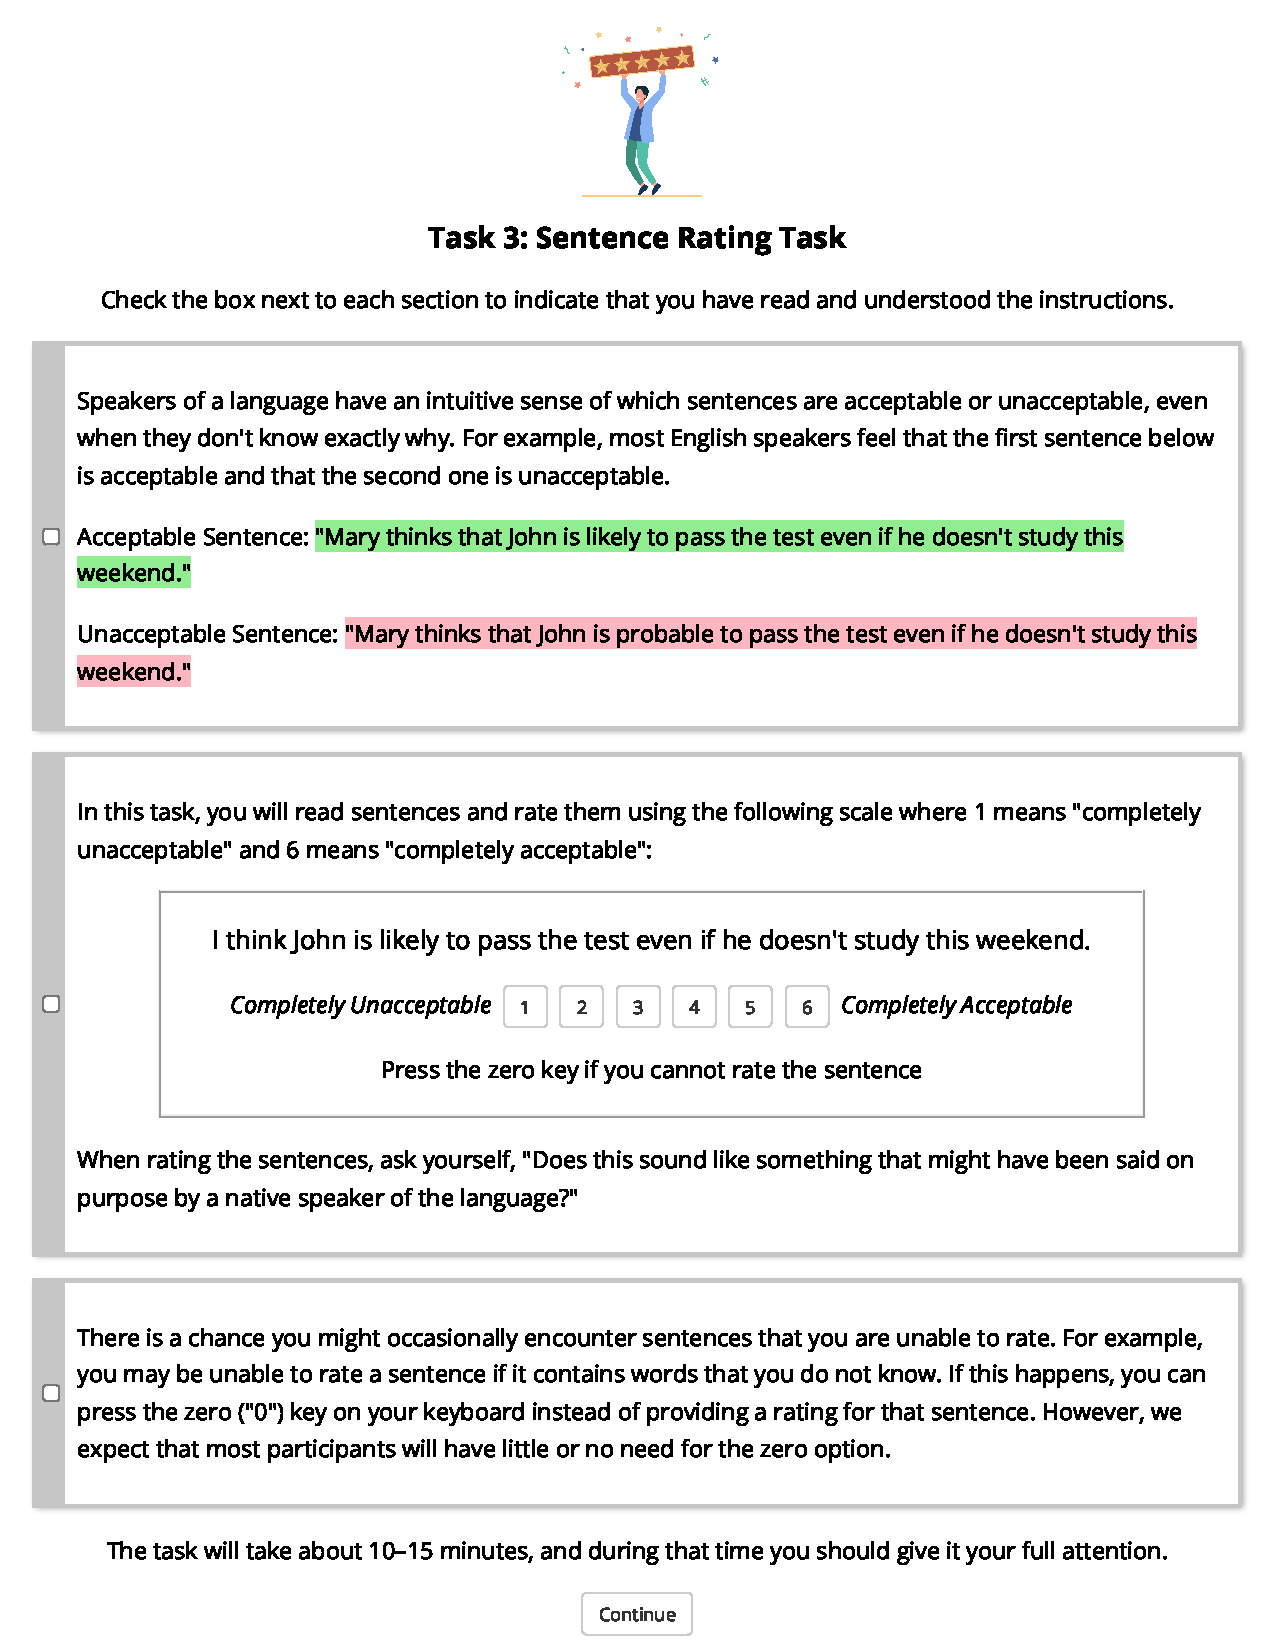
\includegraphics{../materials/instructions/en-05-ajt.pdf}
\newpage

%========================================================%
\section{Korean instructions in the ORC and SRC English acceptability judgment tasks}
%========================================================%

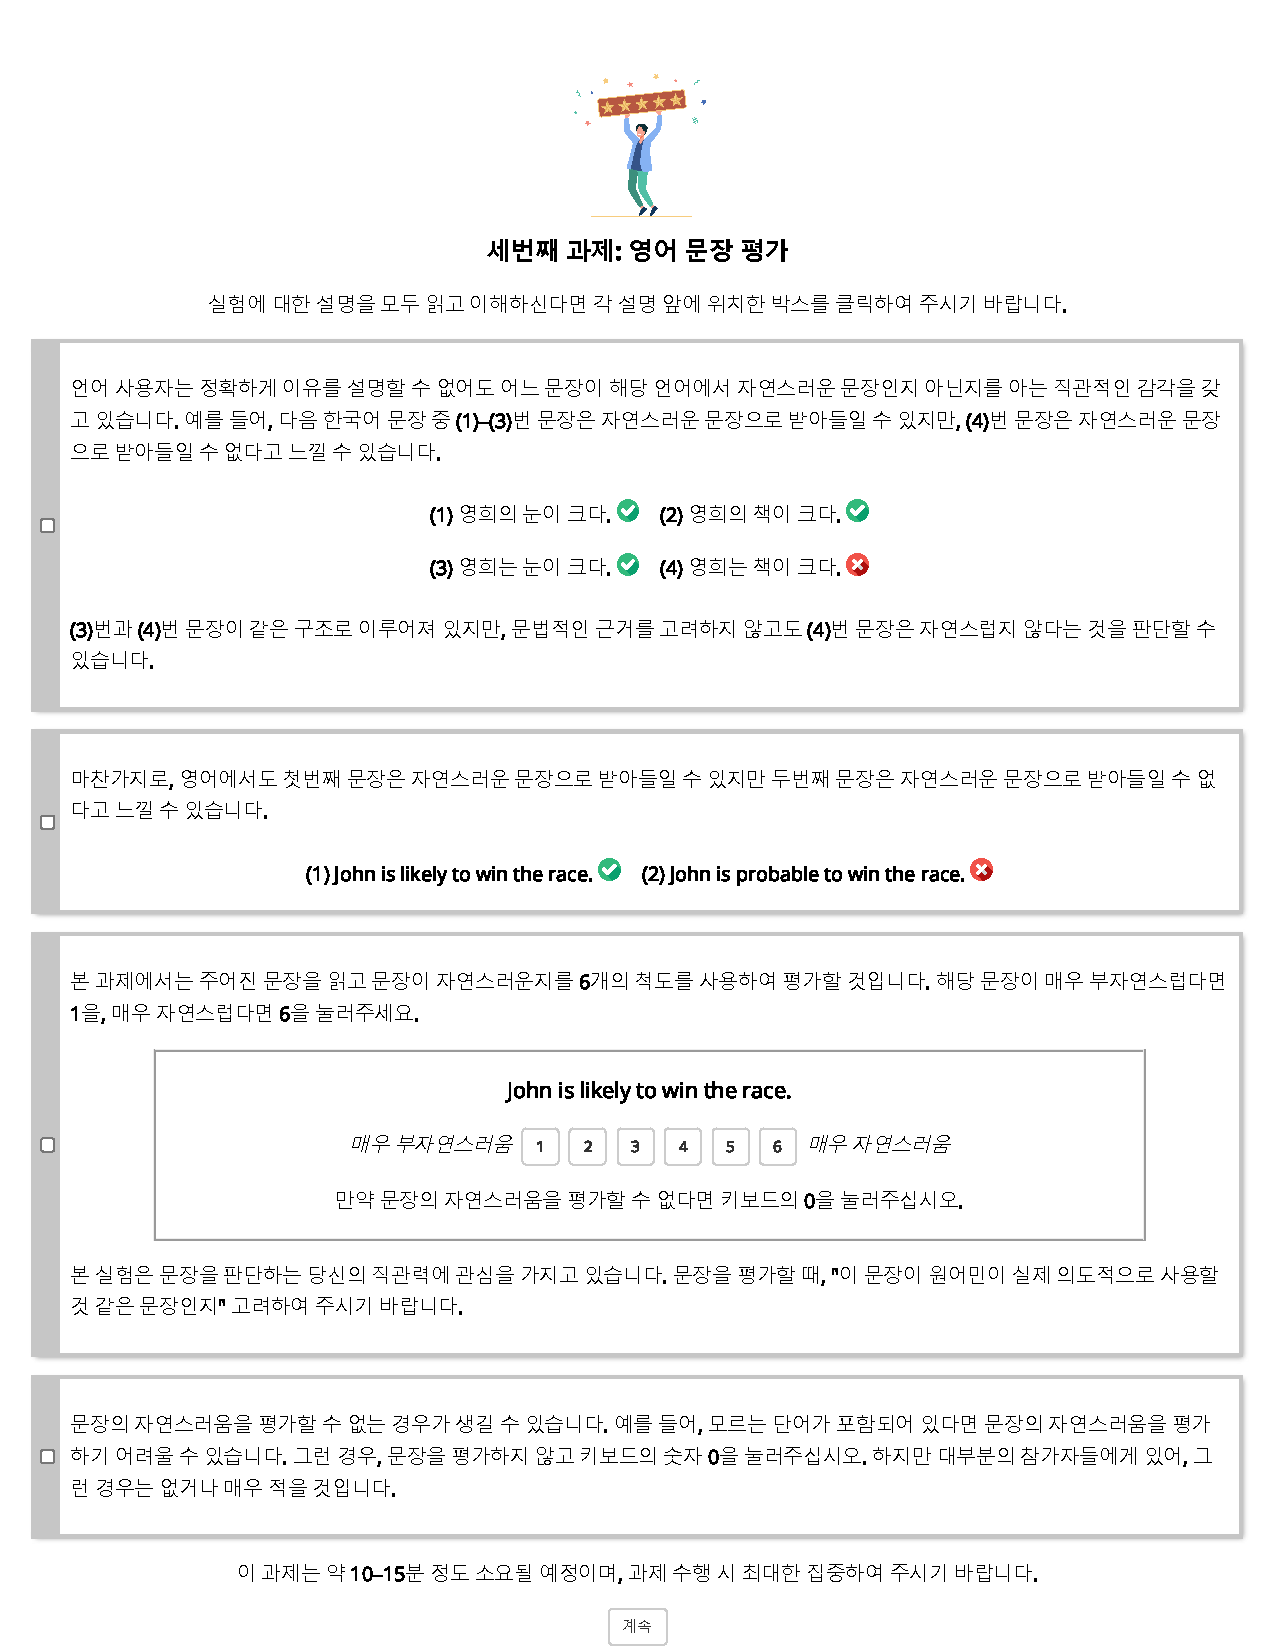
\includegraphics{../materials/instructions/ko-05-ajt.pdf}
\newpage

%========================================================%
\section{Korean instructions in the ORC and SRC Korean acceptability judgment tasks}
%========================================================%

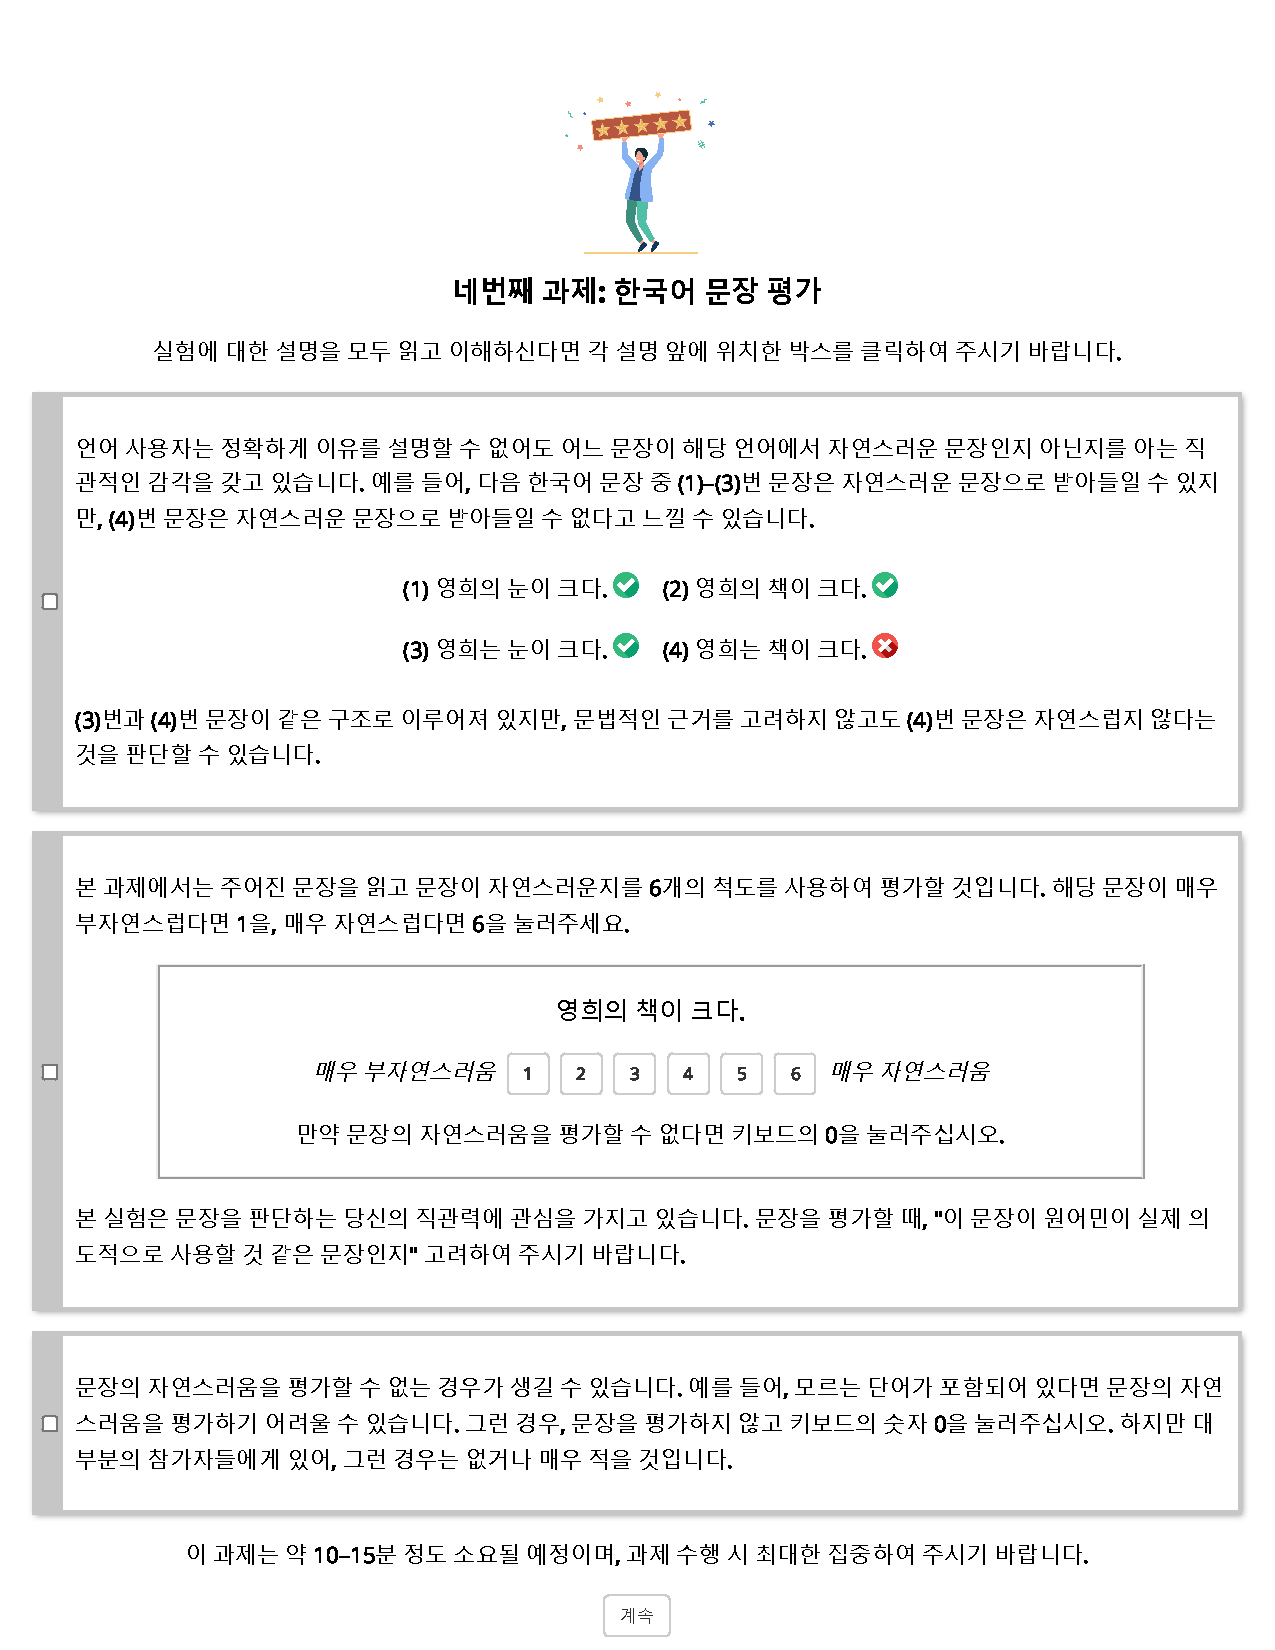
\includegraphics{../materials/instructions/ko-06-ajt.pdf}
\newpage

%========================================================%
\section{Mandarin instructions in the ORC and SRC English acceptability judgment tasks}
%========================================================%

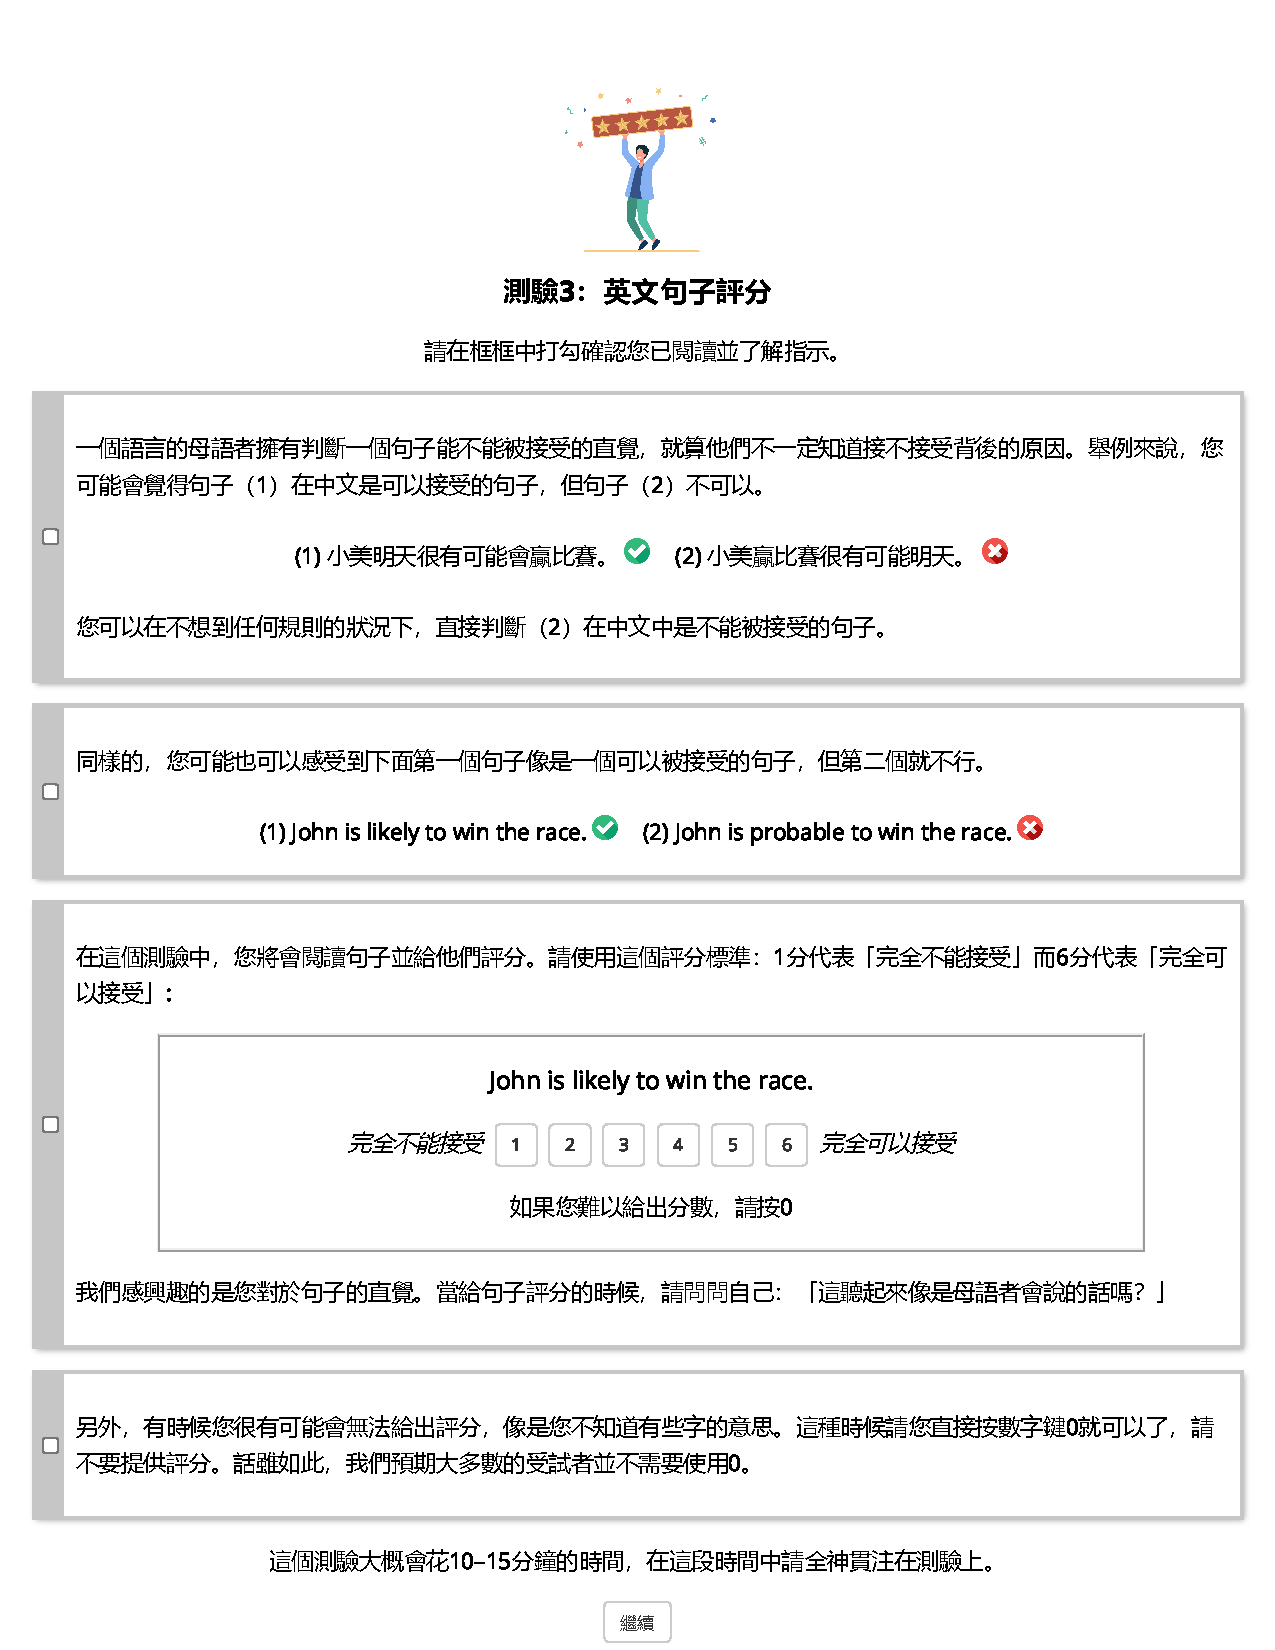
\includegraphics{../materials/instructions/zh-05-ajt.pdf}
\newpage

%========================================================%
\section{Mandarin instructions in the ORC and SRC Mandarin acceptability judgment tasks}
%========================================================%

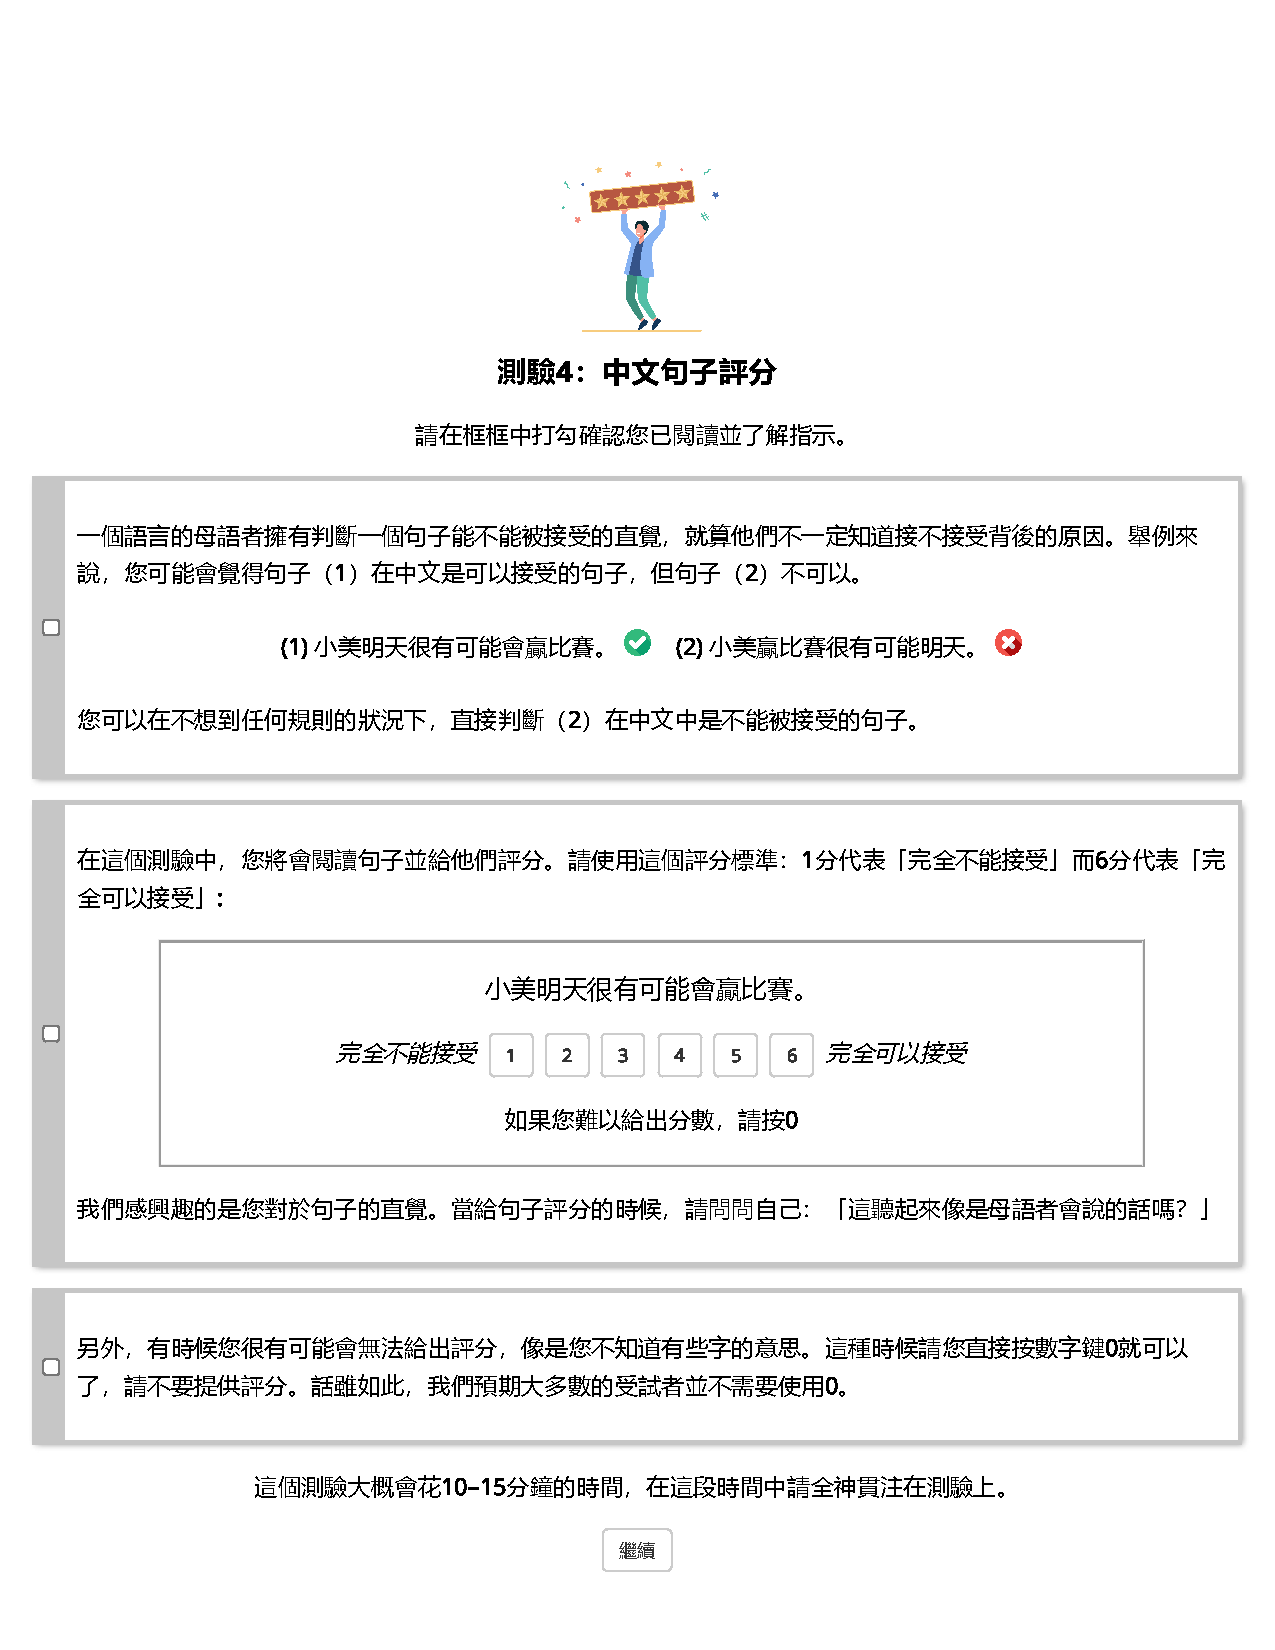
\includegraphics{../materials/instructions/zh-06-ajt.pdf}